\subsection{Thiết kế giao diện}
\subsubsection{Giao diện khách hàng}

% --- NHÓM 1: XÁC THỰC ---

\begin{figure}[H]
    \centering
    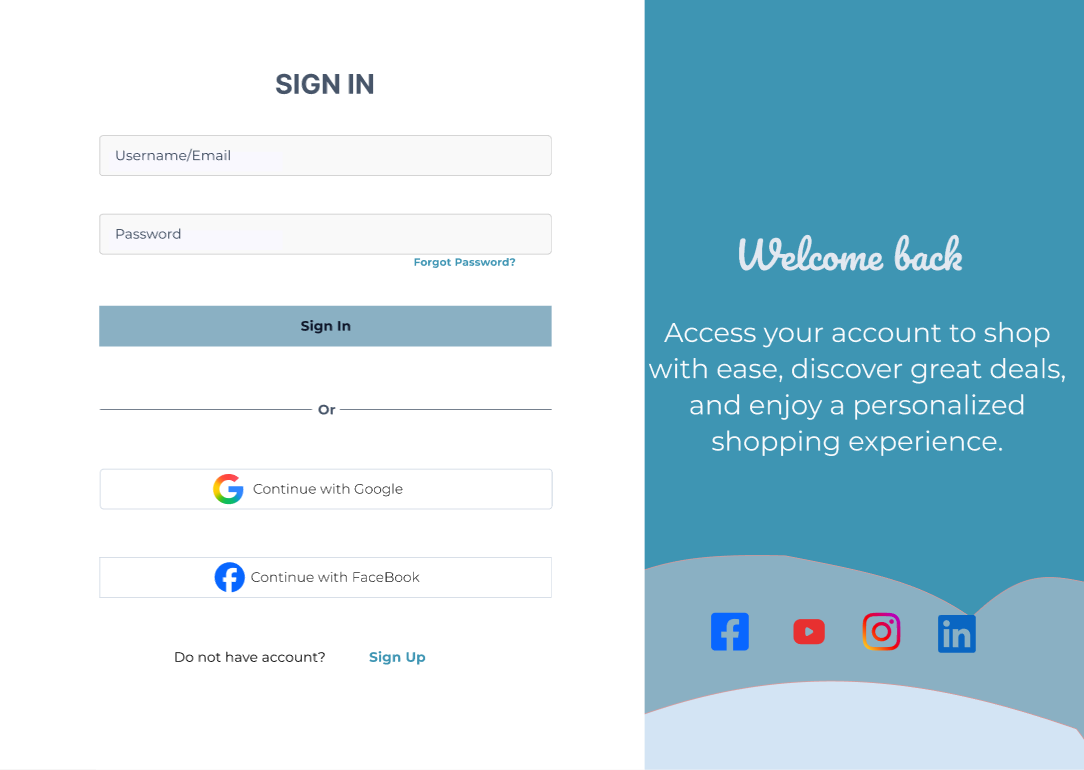
\includegraphics[width=0.8\linewidth]{images/chap6/ui/ui_login.png}
    \vspace{0.5cm}
    \caption{Giao diện Đăng nhập}
    \label{fig:ui_login}
\end{figure}
Giao diện đăng nhập được thiết kế tối giản, tập trung vào form điền thông tin (Email/Tên đăng nhập và Mật khẩu). Hỗ trợ các tính năng tiện ích như “Ghi nhớ đăng nhập” và liên kết nhanh đến trang “Quên mật khẩu” hoặc “Đăng ký” cho người dùng mới.

% --- NHÓM 2: TRANG CHỦ & DUYỆT SẢN PHẨM ---

\begin{figure}[H]
    \centering
    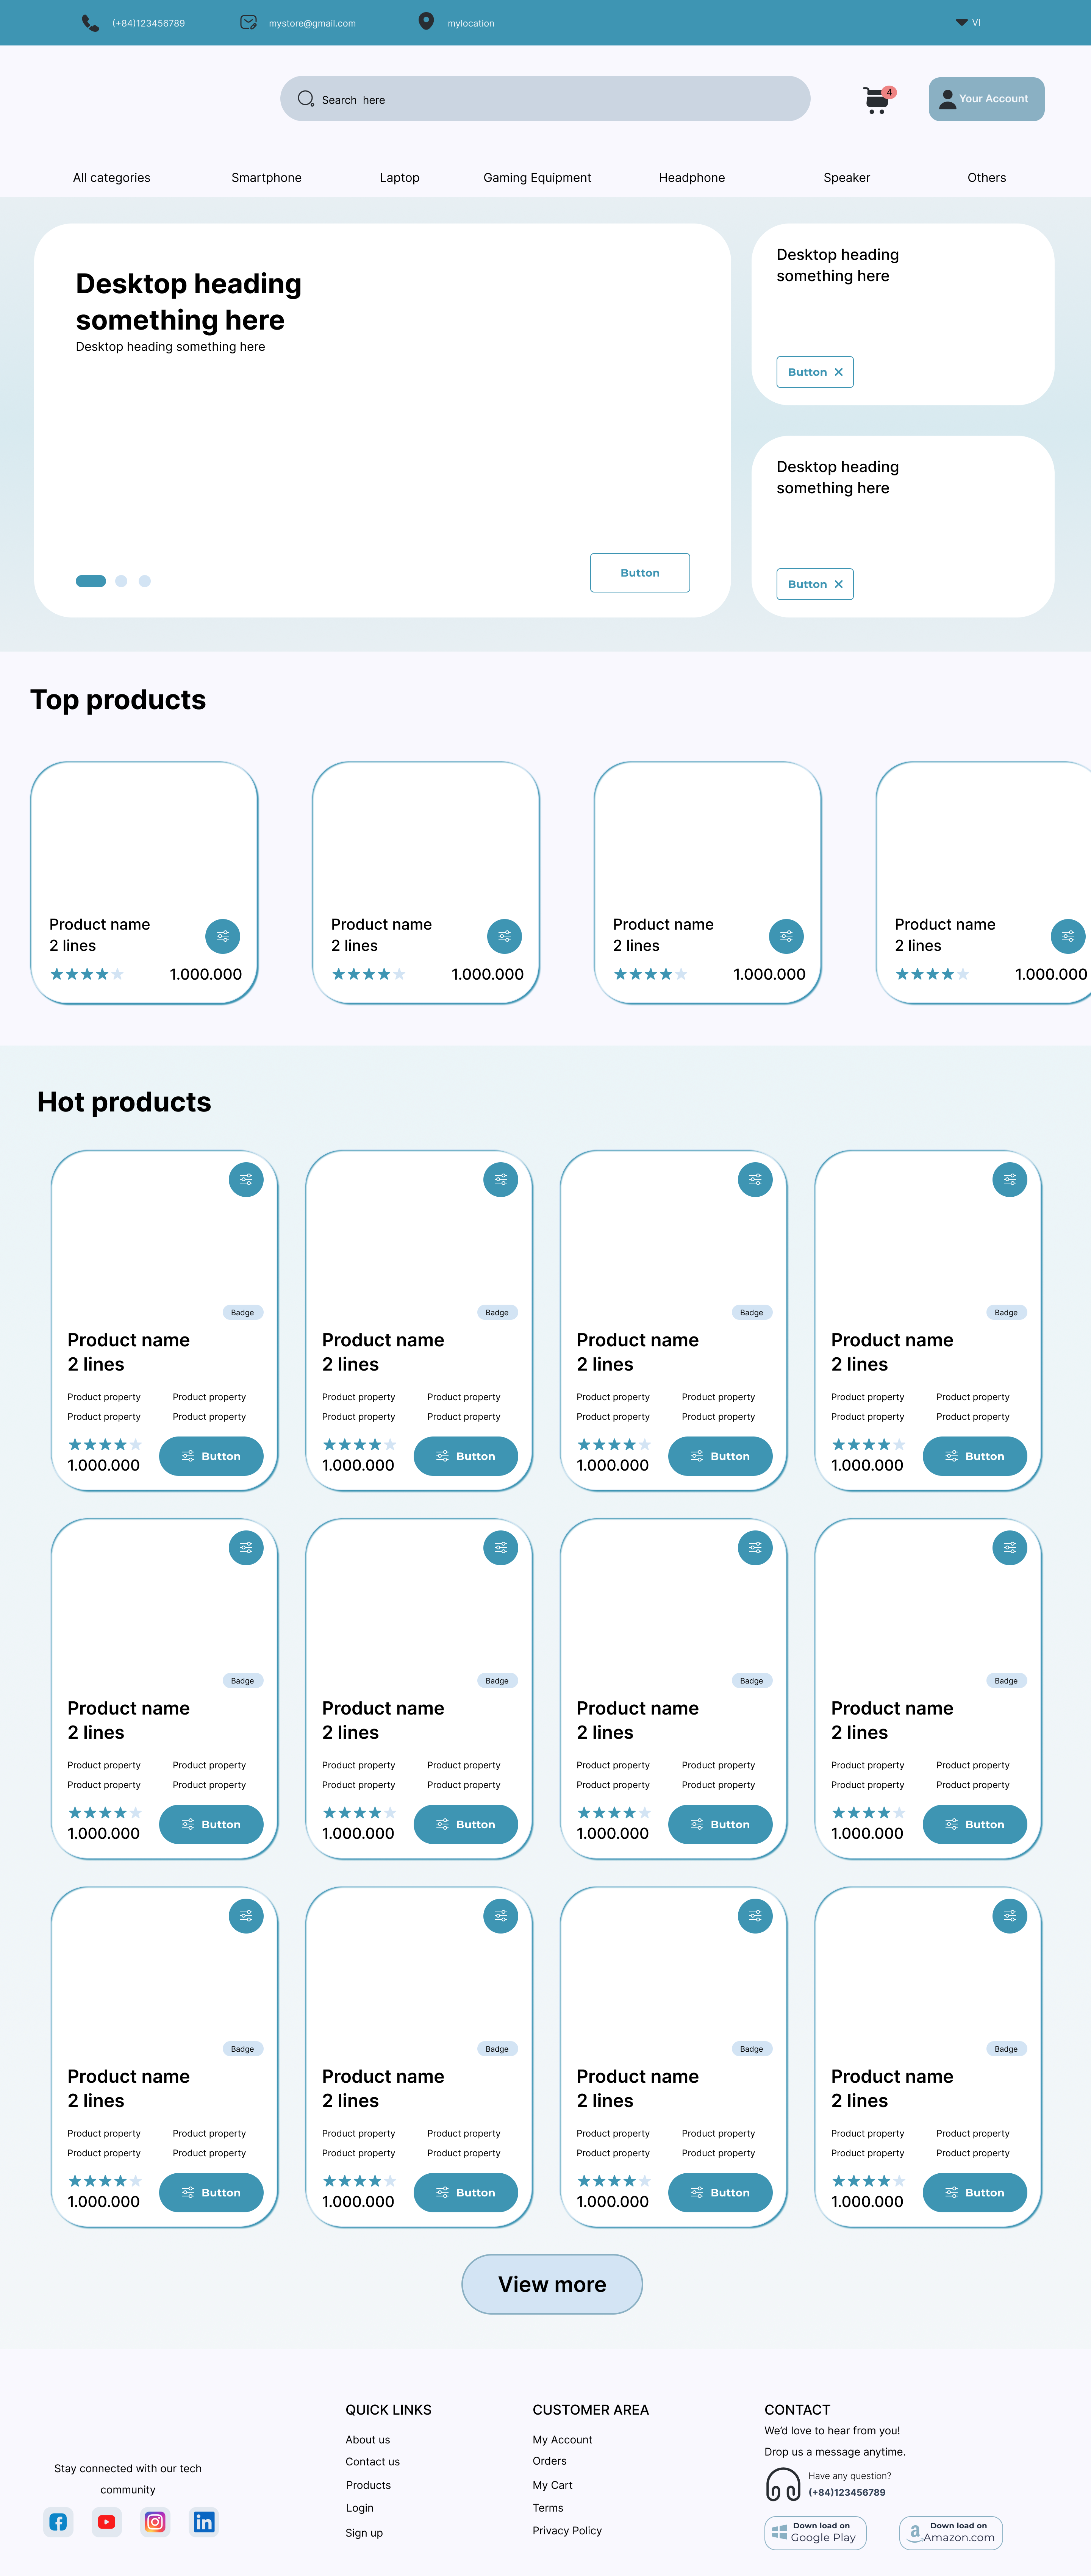
\includegraphics[width=0.6\linewidth]{images/chap6/ui/ui_home.png}
    \vspace{0.5cm}
    \caption{Giao diện Trang chủ (Home Page)}
    \label{fig:ui_home}
\end{figure}
Trang chủ đóng vai trò trung tâm điều hướng của hệ thống, hiển thị các banner khuyến mãi nổi bật nhằm thu hút sự chú ý của người dùng. Các danh mục sản phẩm được phân chia rõ ràng, kết hợp với khu vực gợi ý như “Sản phẩm bán chạy” hoặc “Hàng mới về” để hỗ trợ người dùng khám phá nhanh các sản phẩm phù hợp.

\begin{figure}[H]
    \centering
    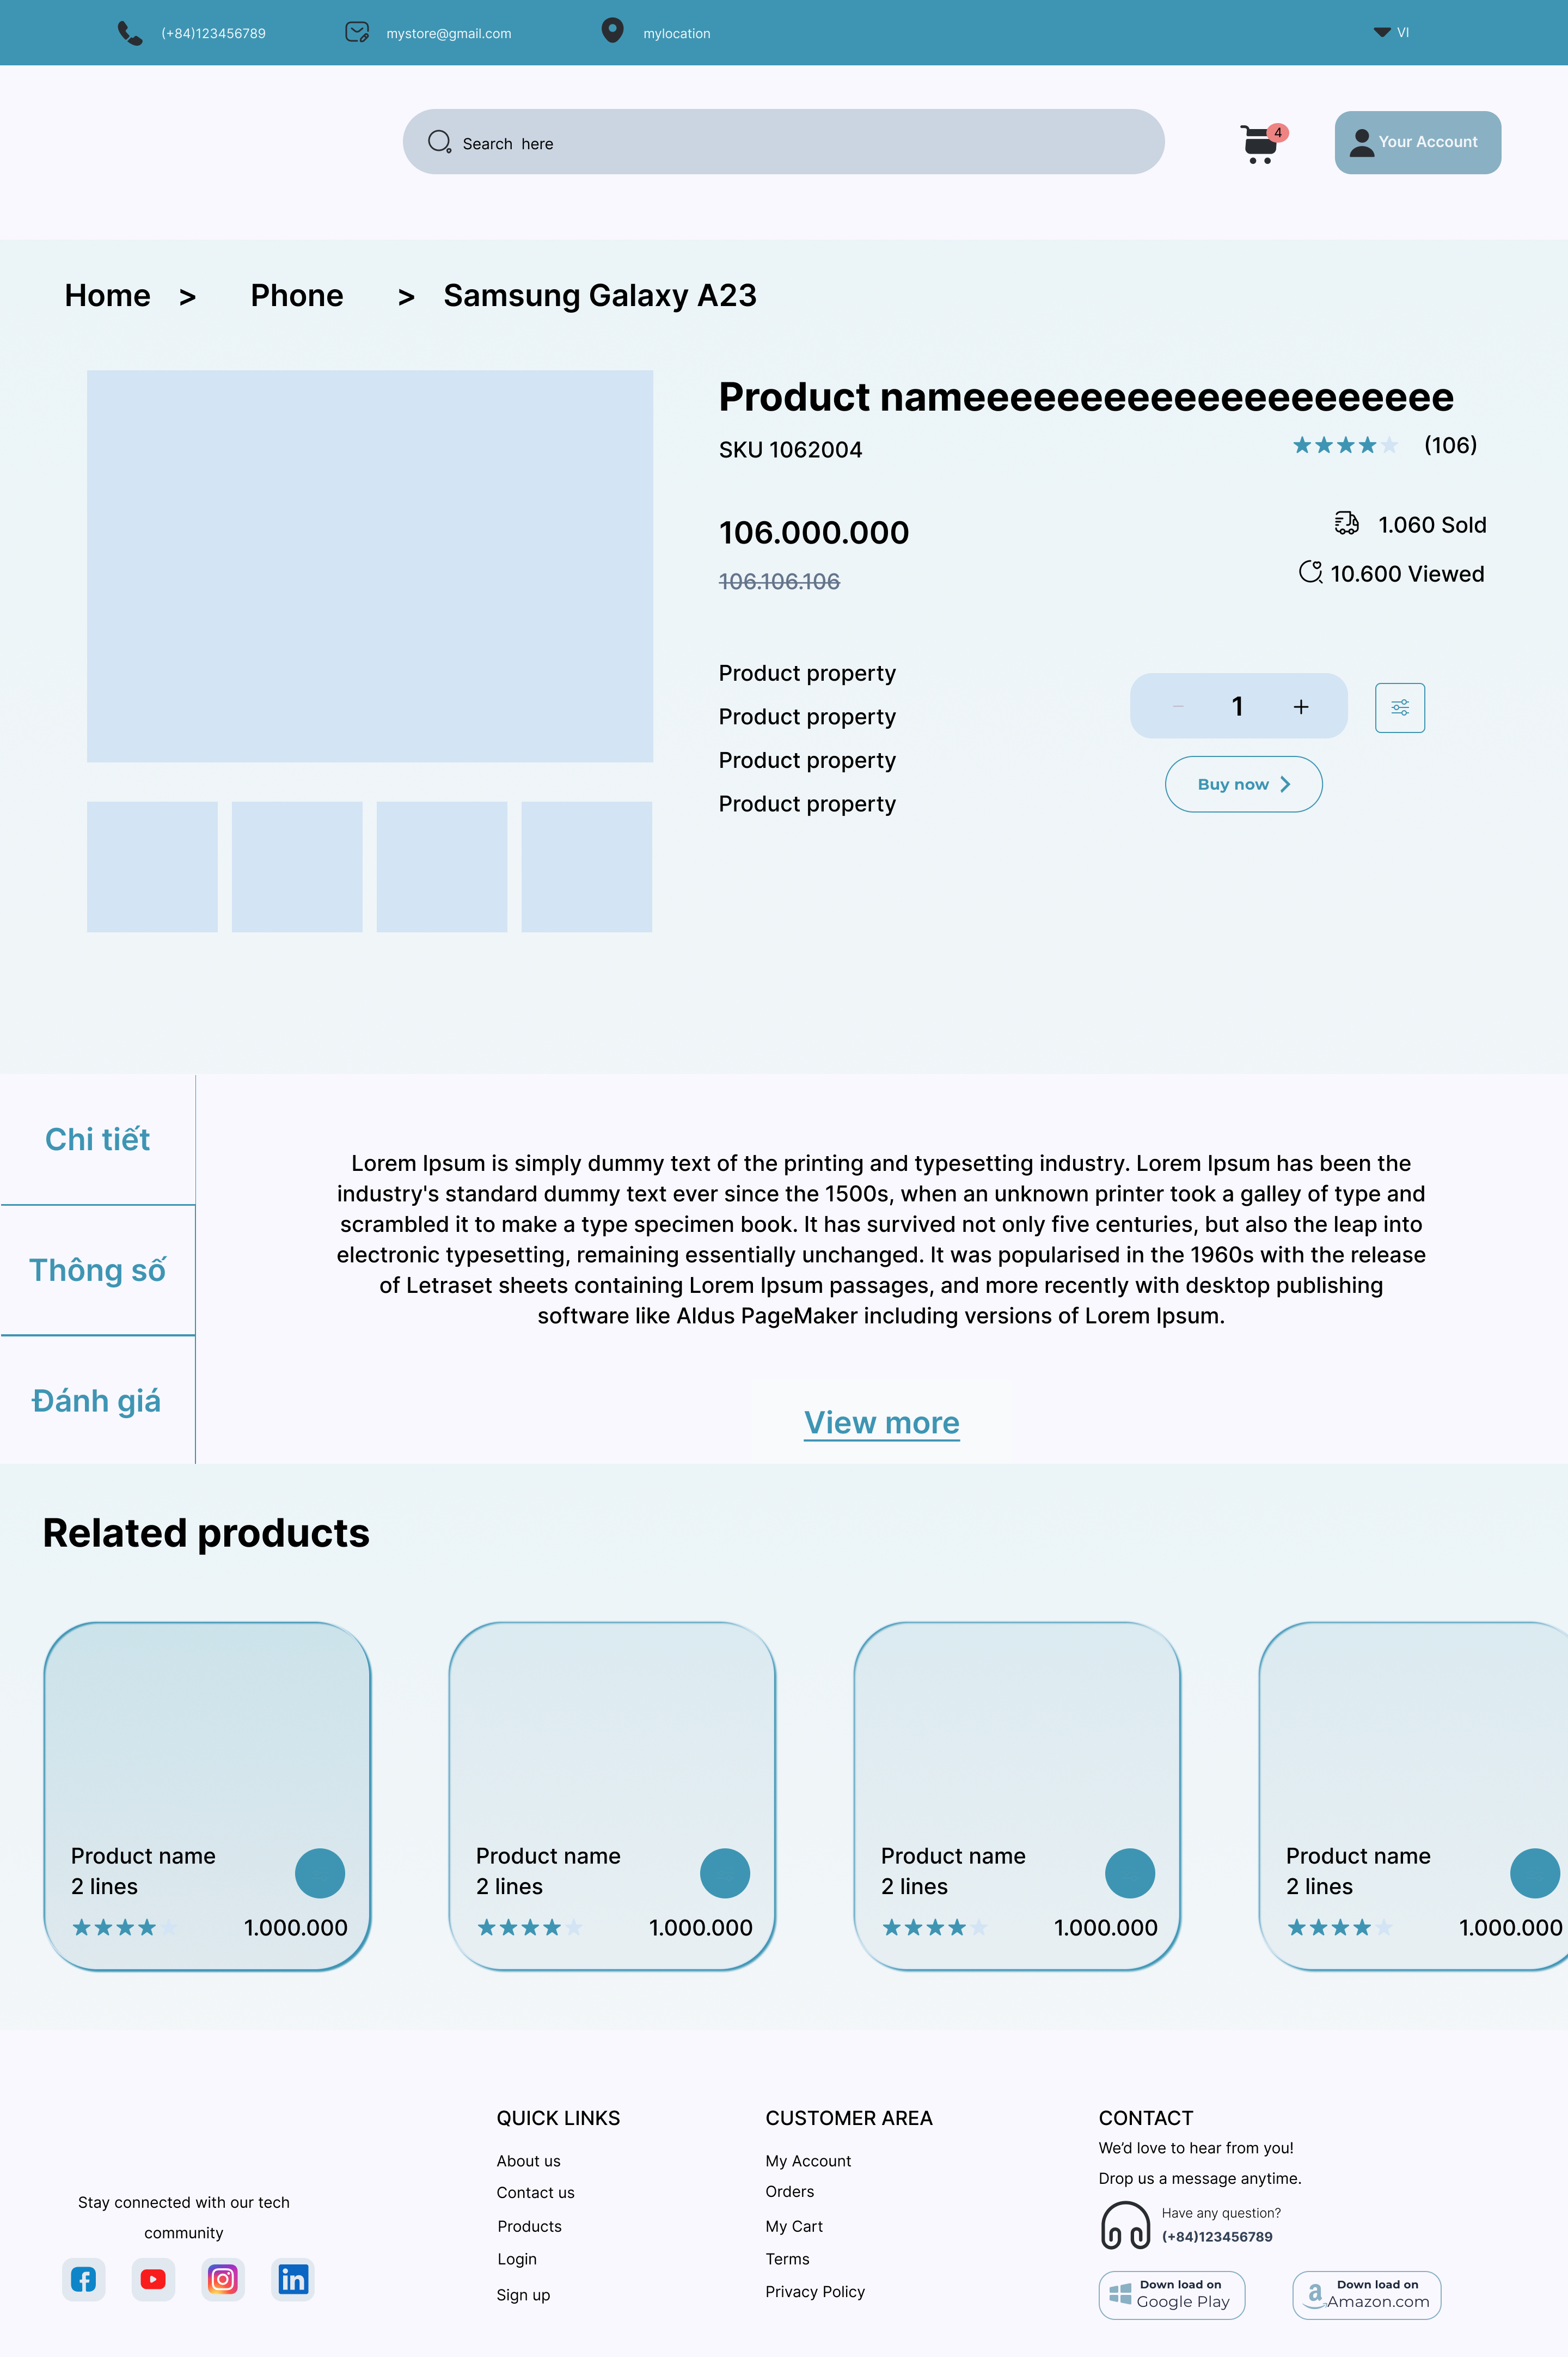
\includegraphics[width=0.9\linewidth]{images/chap6/ui/ui_product_filter.png}
    \vspace{0.5cm}
    \caption{Giao diện Danh sách và Bộ lọc sản phẩm}
    \label{fig:ui_filter}
\end{figure}
Giao diện danh sách sản phẩm tích hợp bộ lọc nâng cao, cho phép người dùng thu hẹp kết quả tìm kiếm theo nhiều tiêu chí như khoảng giá, thương hiệu, mức đánh giá và loại sản phẩm. Cách bố trí dạng sidebar giúp thao tác lọc nhanh mà không làm gián đoạn trải nghiệm duyệt sản phẩm.

\begin{figure}[H]
    \centering
    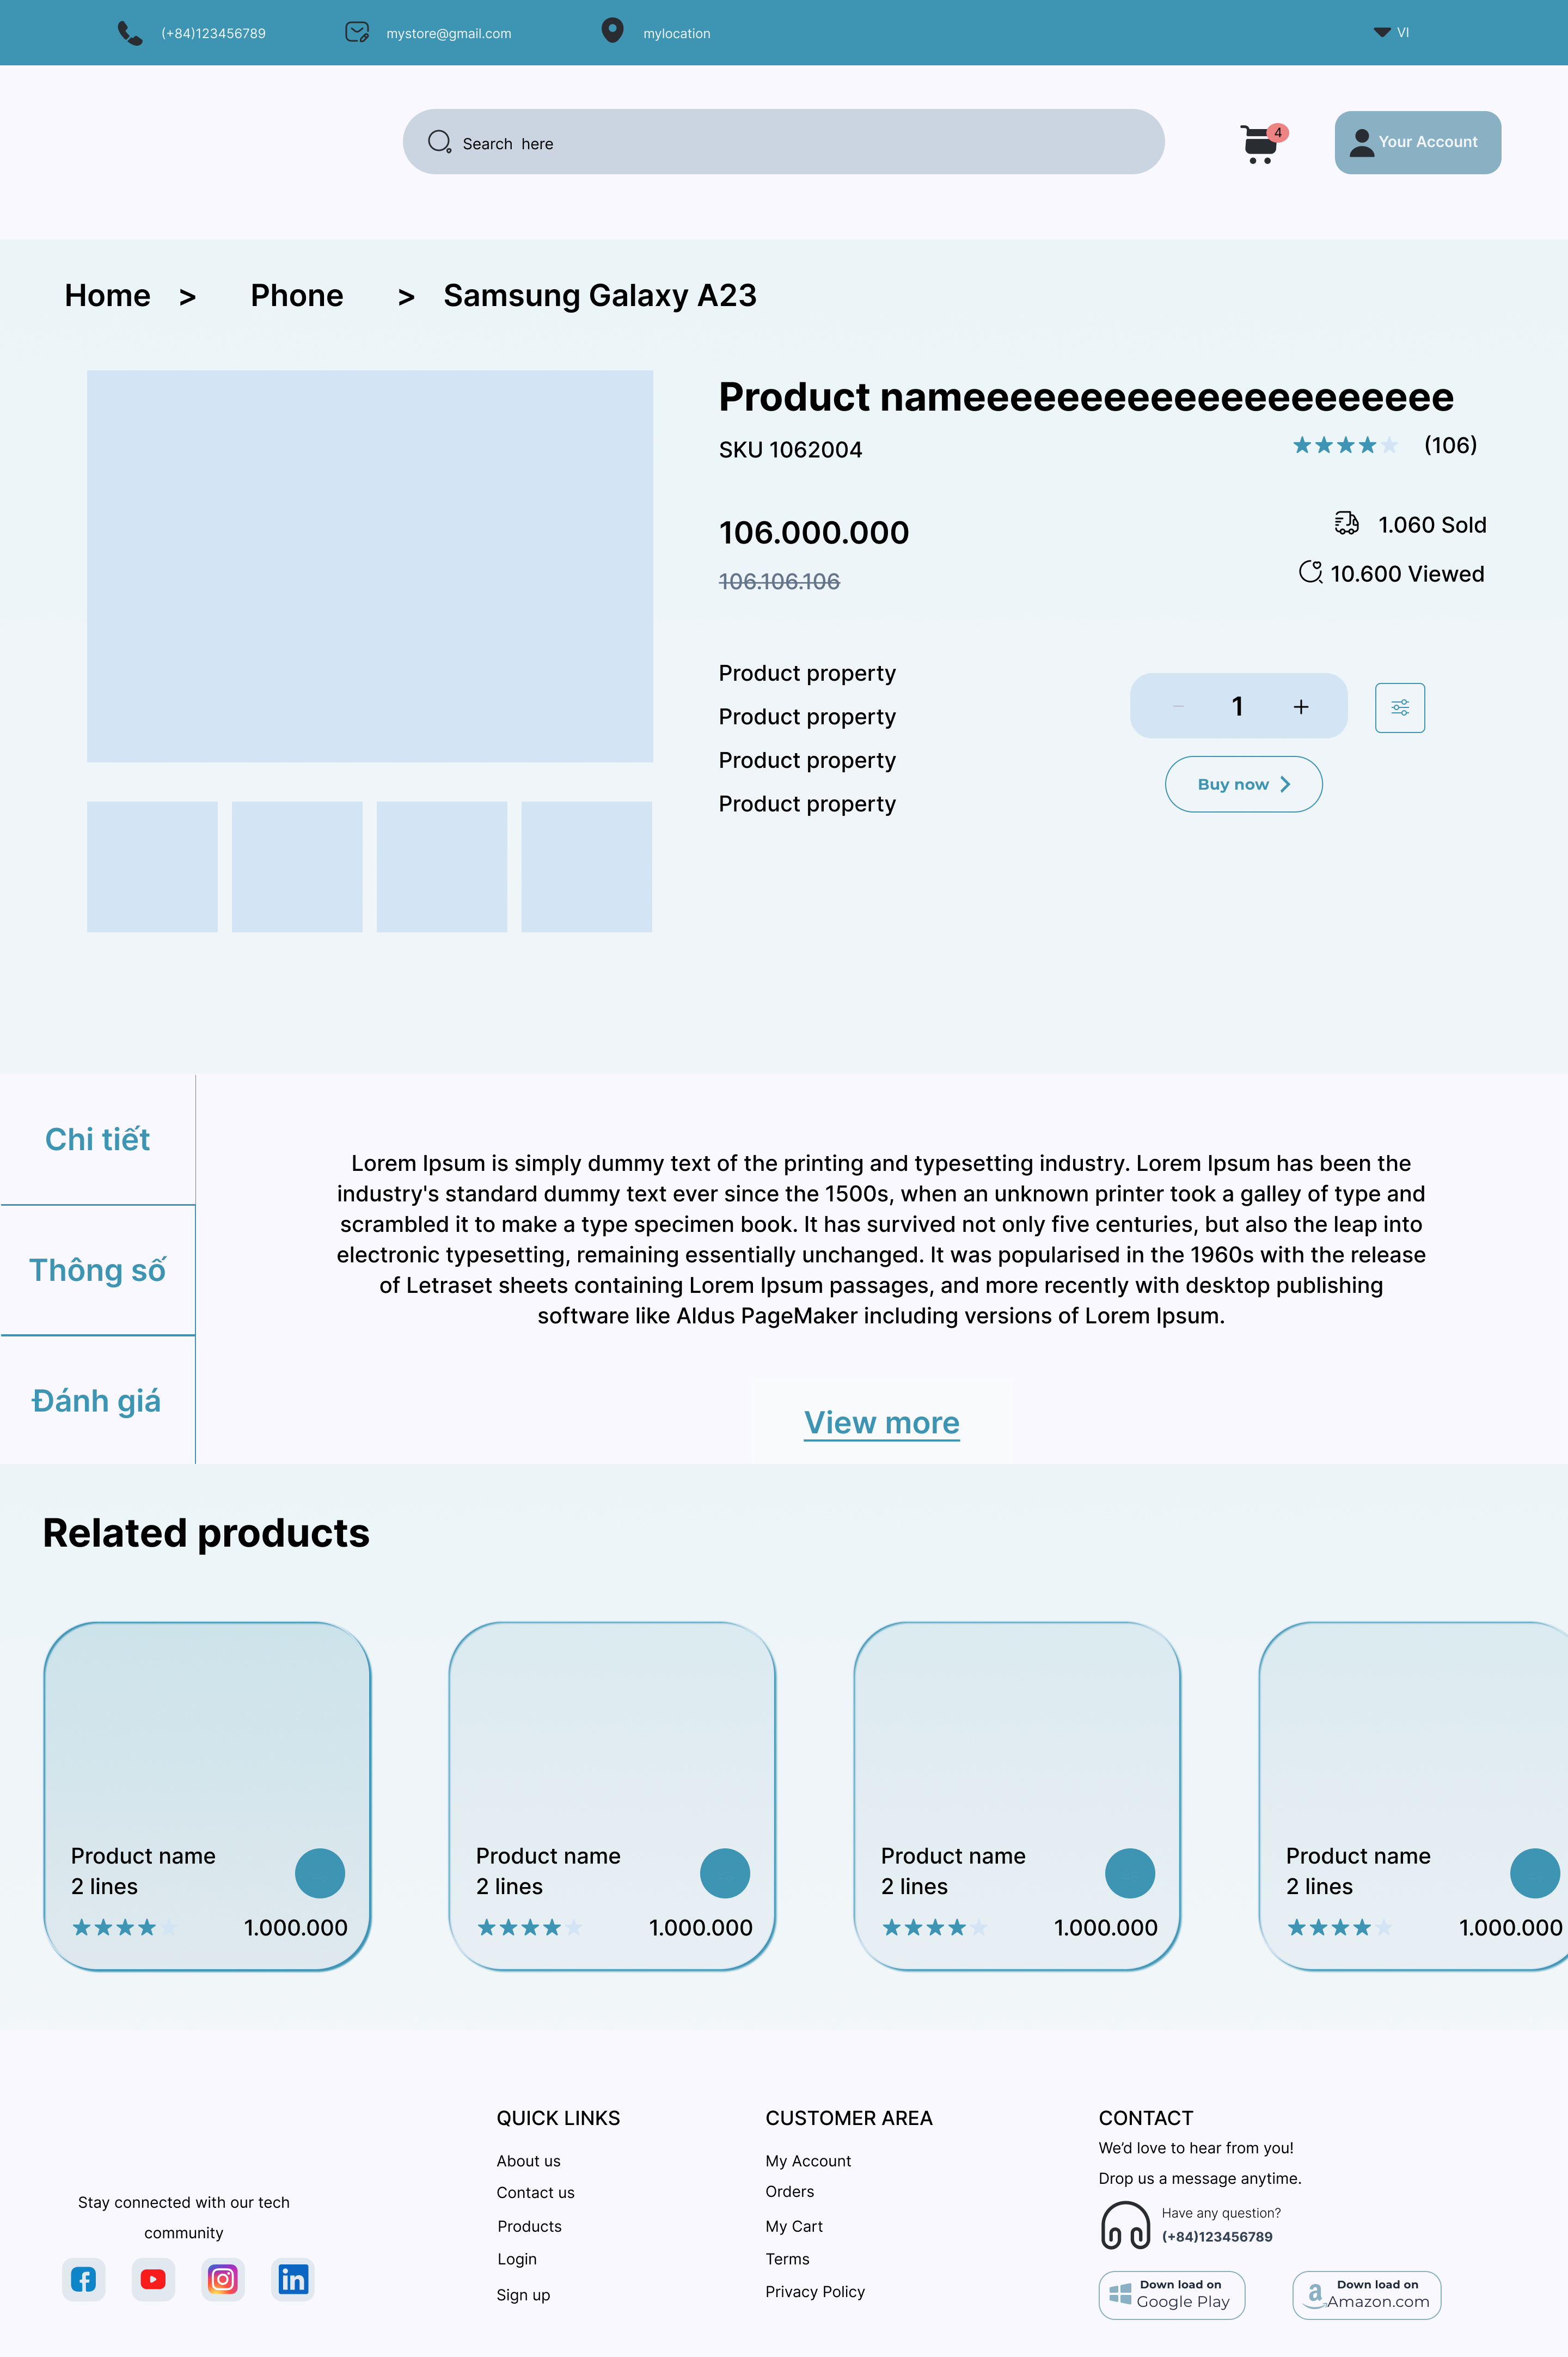
\includegraphics[width=0.9\linewidth]{images/chap6/ui/ui_product_detail.png}
    \vspace{0.5cm}
    \caption{Giao diện Chi tiết sản phẩm}
    \label{fig:ui_product_detail}
\end{figure}
Trang chi tiết sản phẩm cung cấp đầy đủ thông tin cần thiết trước khi mua hàng, bao gồm hình ảnh độ phân giải cao, thông số kỹ thuật, giá bán, tình trạng tồn kho và các tùy chọn phiên bản. Nút “Thêm vào giỏ hàng” được đặt ở vị trí nổi bật nhằm thúc đẩy hành động mua của người dùng.

% --- NHÓM 3: MUA HÀNG & THANH TOÁN ---

\begin{figure}[H]
    \centering
    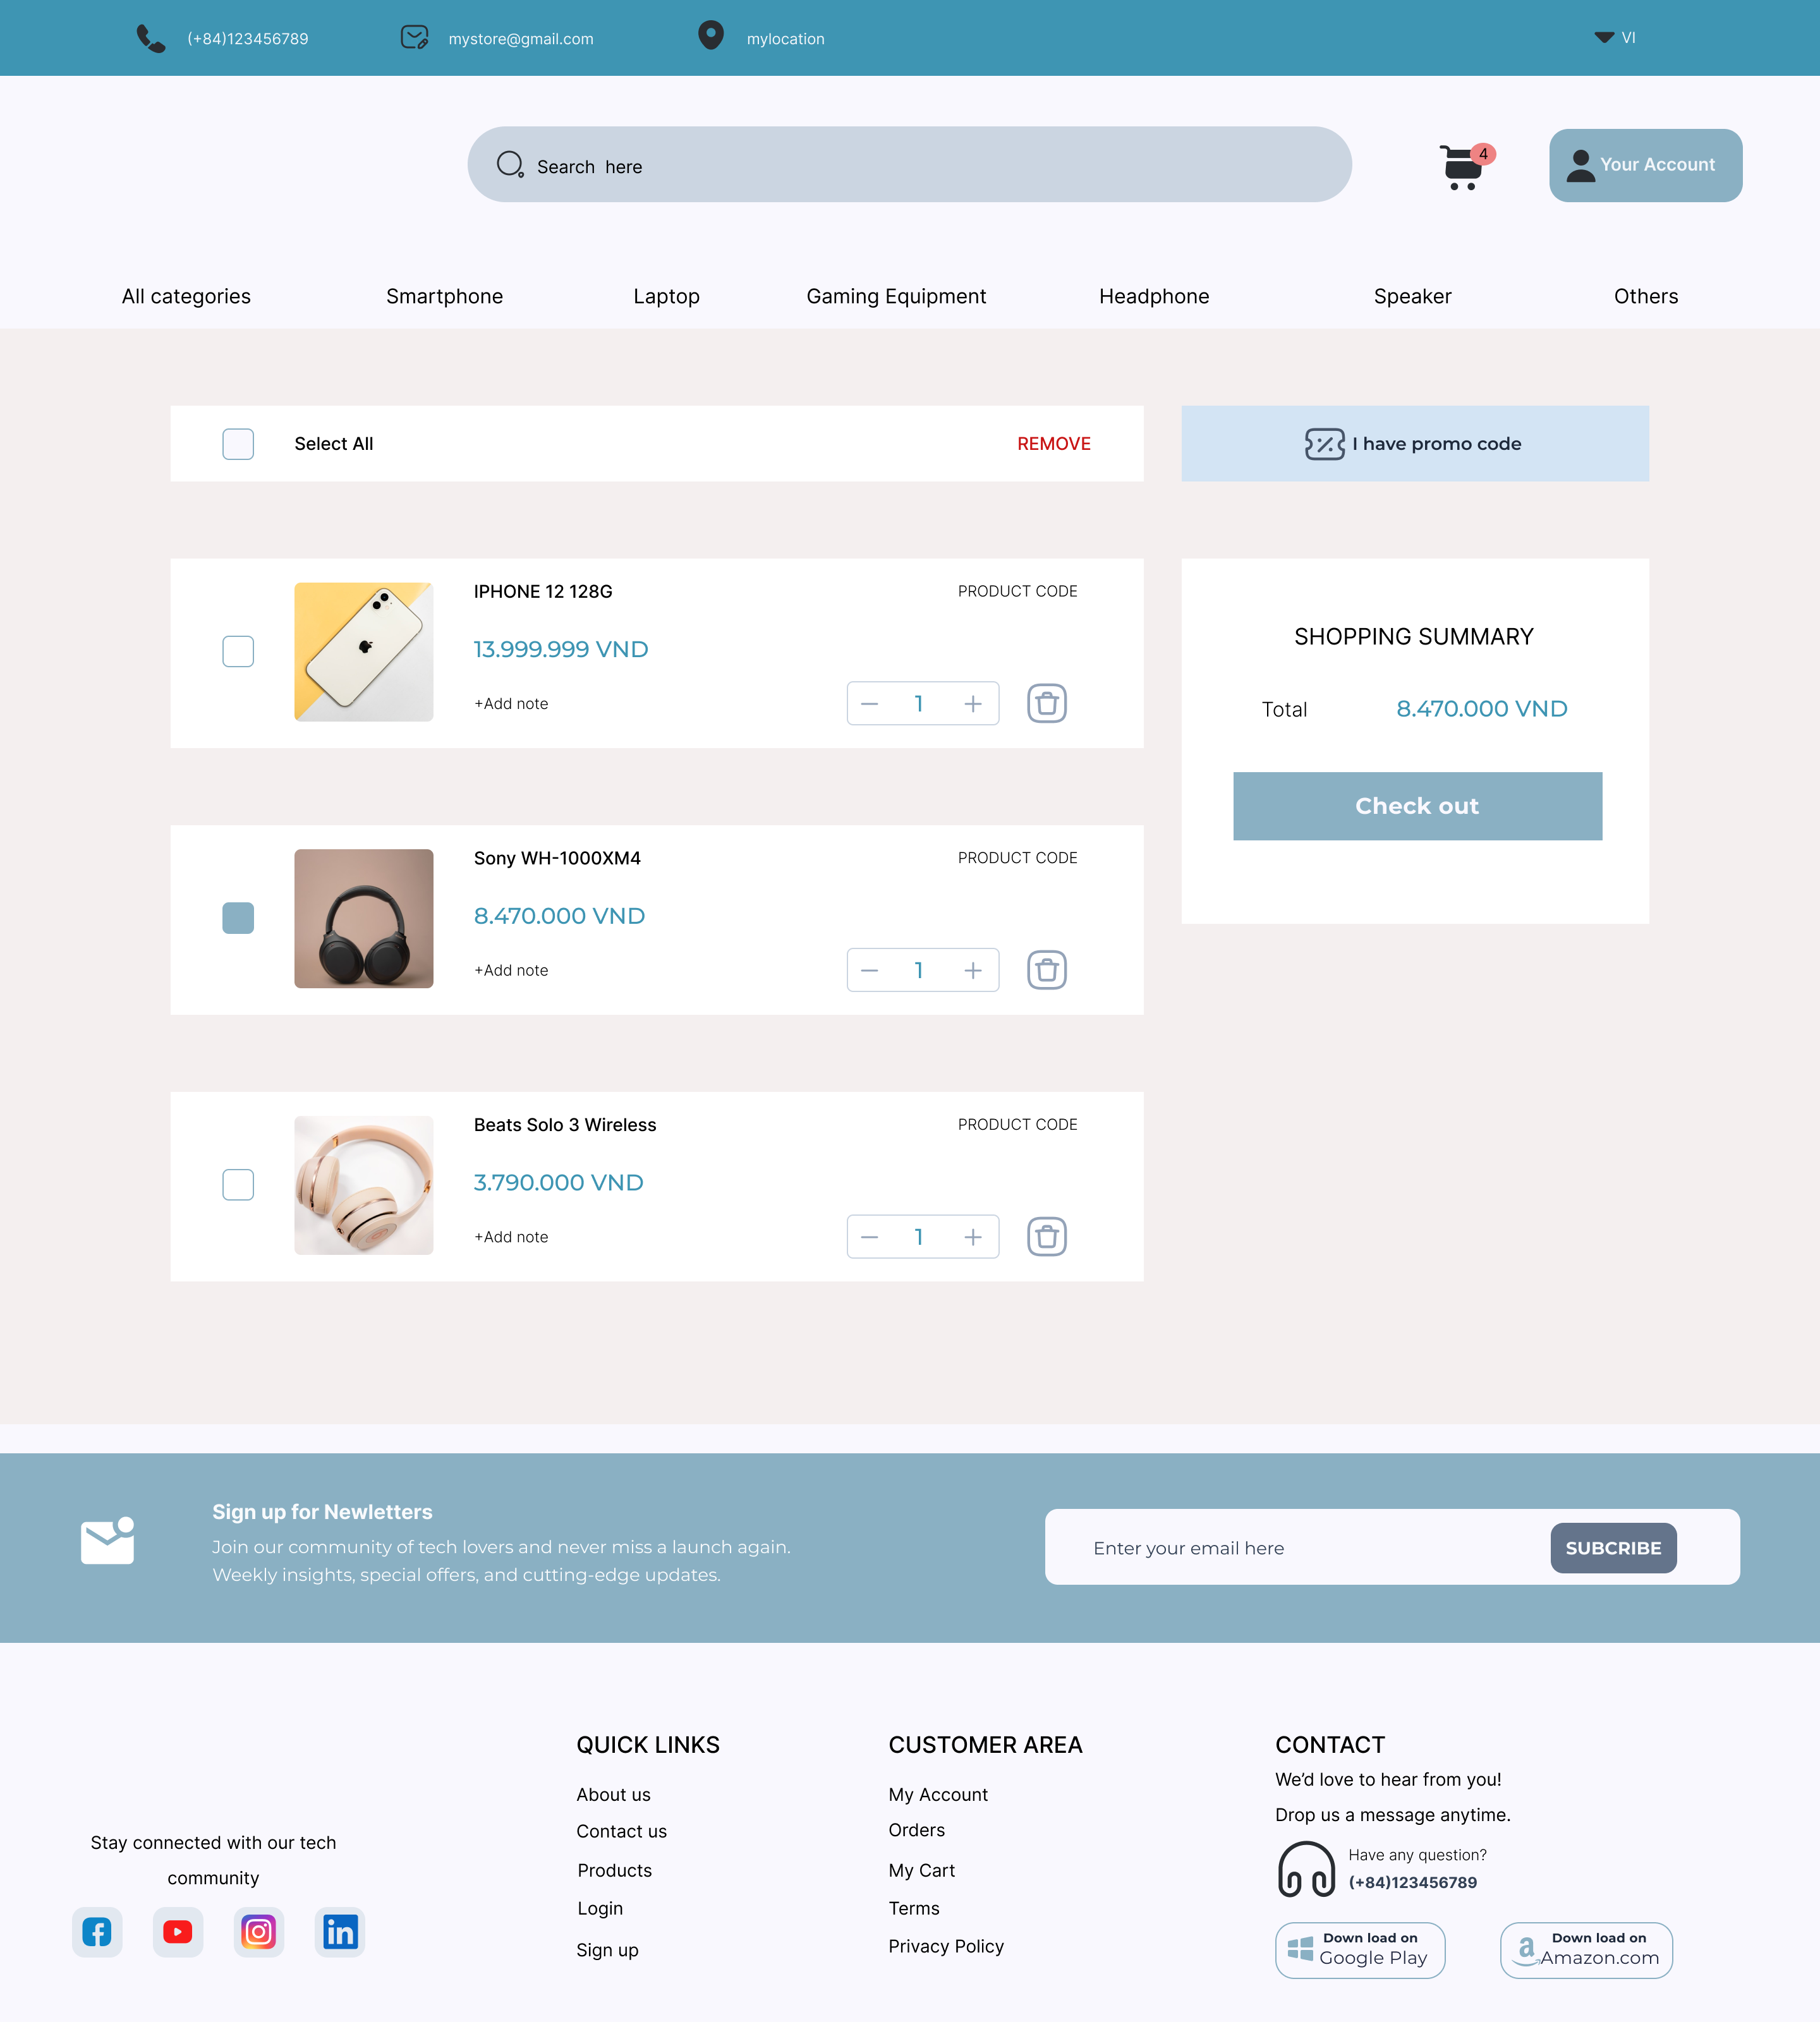
\includegraphics[width=0.9\linewidth]{images/chap6/ui/ui_cart.png}
    \vspace{0.5cm}
    \caption{Giao diện Giỏ hàng}
    \label{fig:ui_cart}
\end{figure}
Giao diện giỏ hàng cho phép người dùng kiểm tra lại các sản phẩm đã chọn, điều chỉnh số lượng hoặc loại bỏ sản phẩm không cần thiết. Tổng giá trị đơn hàng được cập nhật theo thời gian thực để người dùng dễ dàng theo dõi chi phí.

\begin{figure}[H]
    \centering
    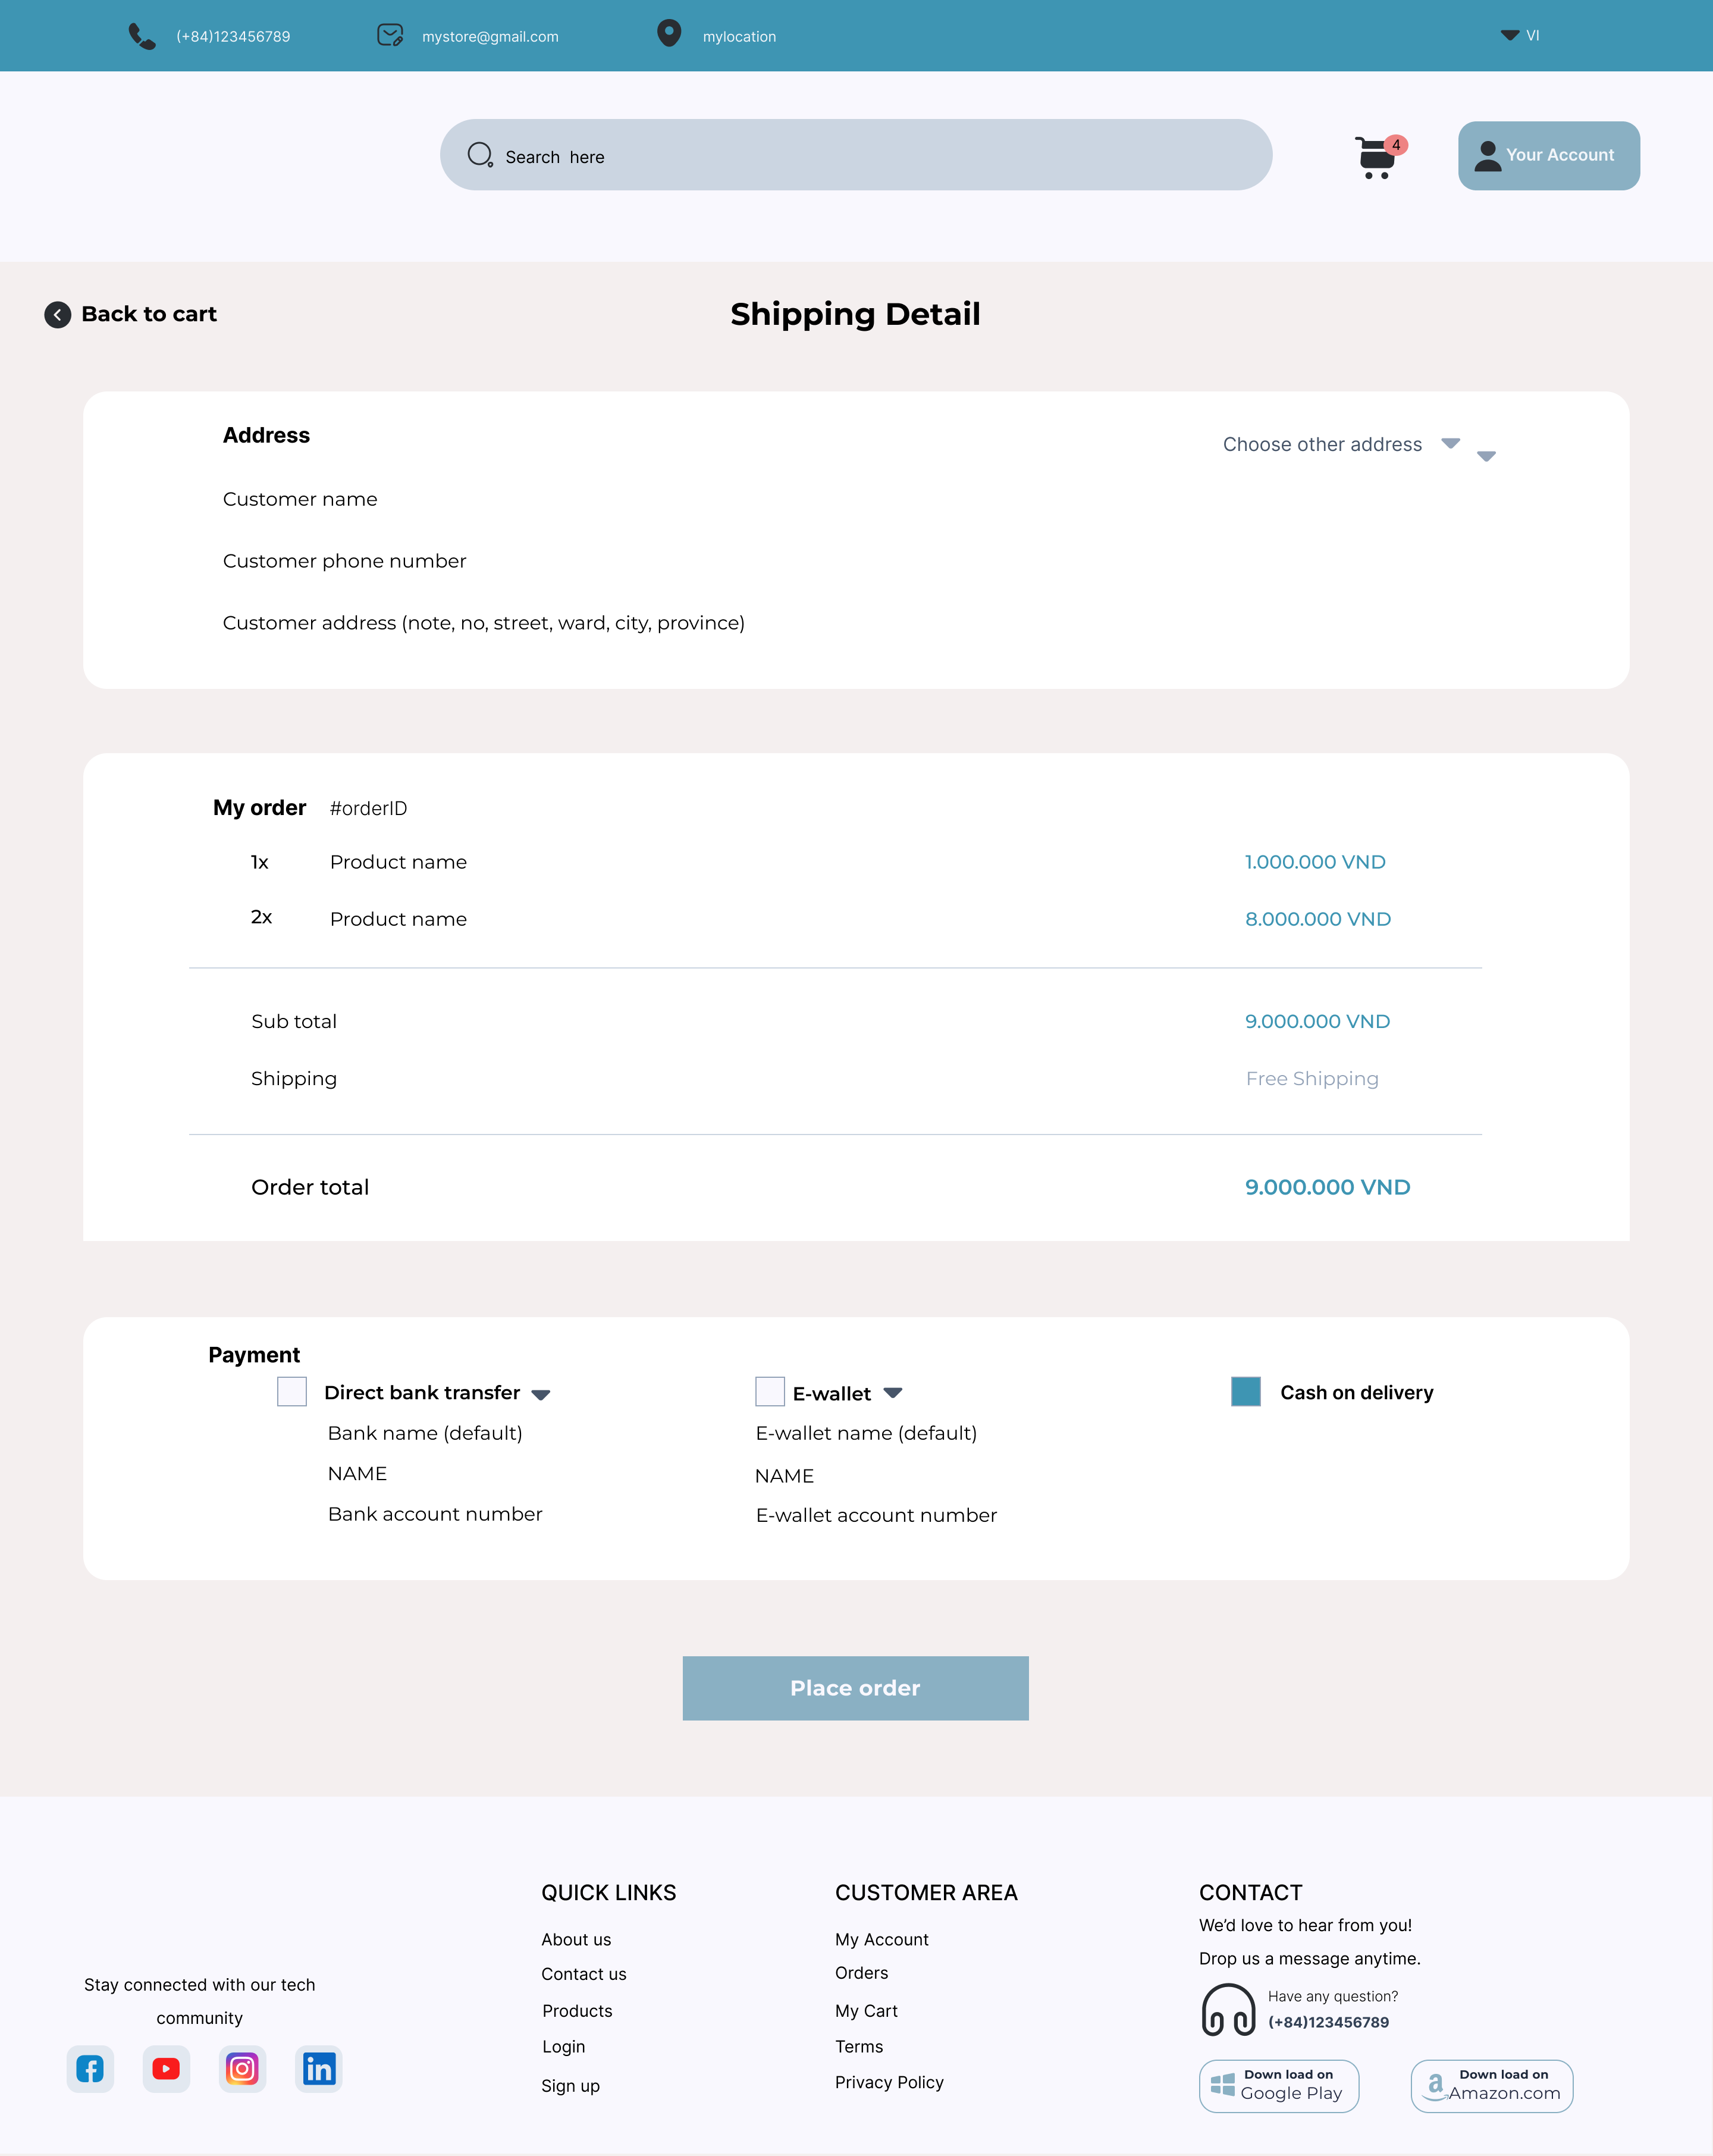
\includegraphics[width=0.9\linewidth]{images/chap6/ui/ui_shipping_detail.png}
    \vspace{0.5cm}
    \caption{Giao diện Thông tin giao hàng}
    \label{fig:ui_shipping}
\end{figure}
Đây là bước người dùng nhập địa chỉ nhận hàng và lựa chọn phương thức vận chuyển. Hệ thống hỗ trợ gợi ý các địa chỉ đã lưu nhằm rút ngắn thời gian thao tác và giảm sai sót khi đặt hàng.

% --- NHÓM 4: QUẢN LÝ TÀI KHOẢN ---

\begin{figure}[H]
    \centering
    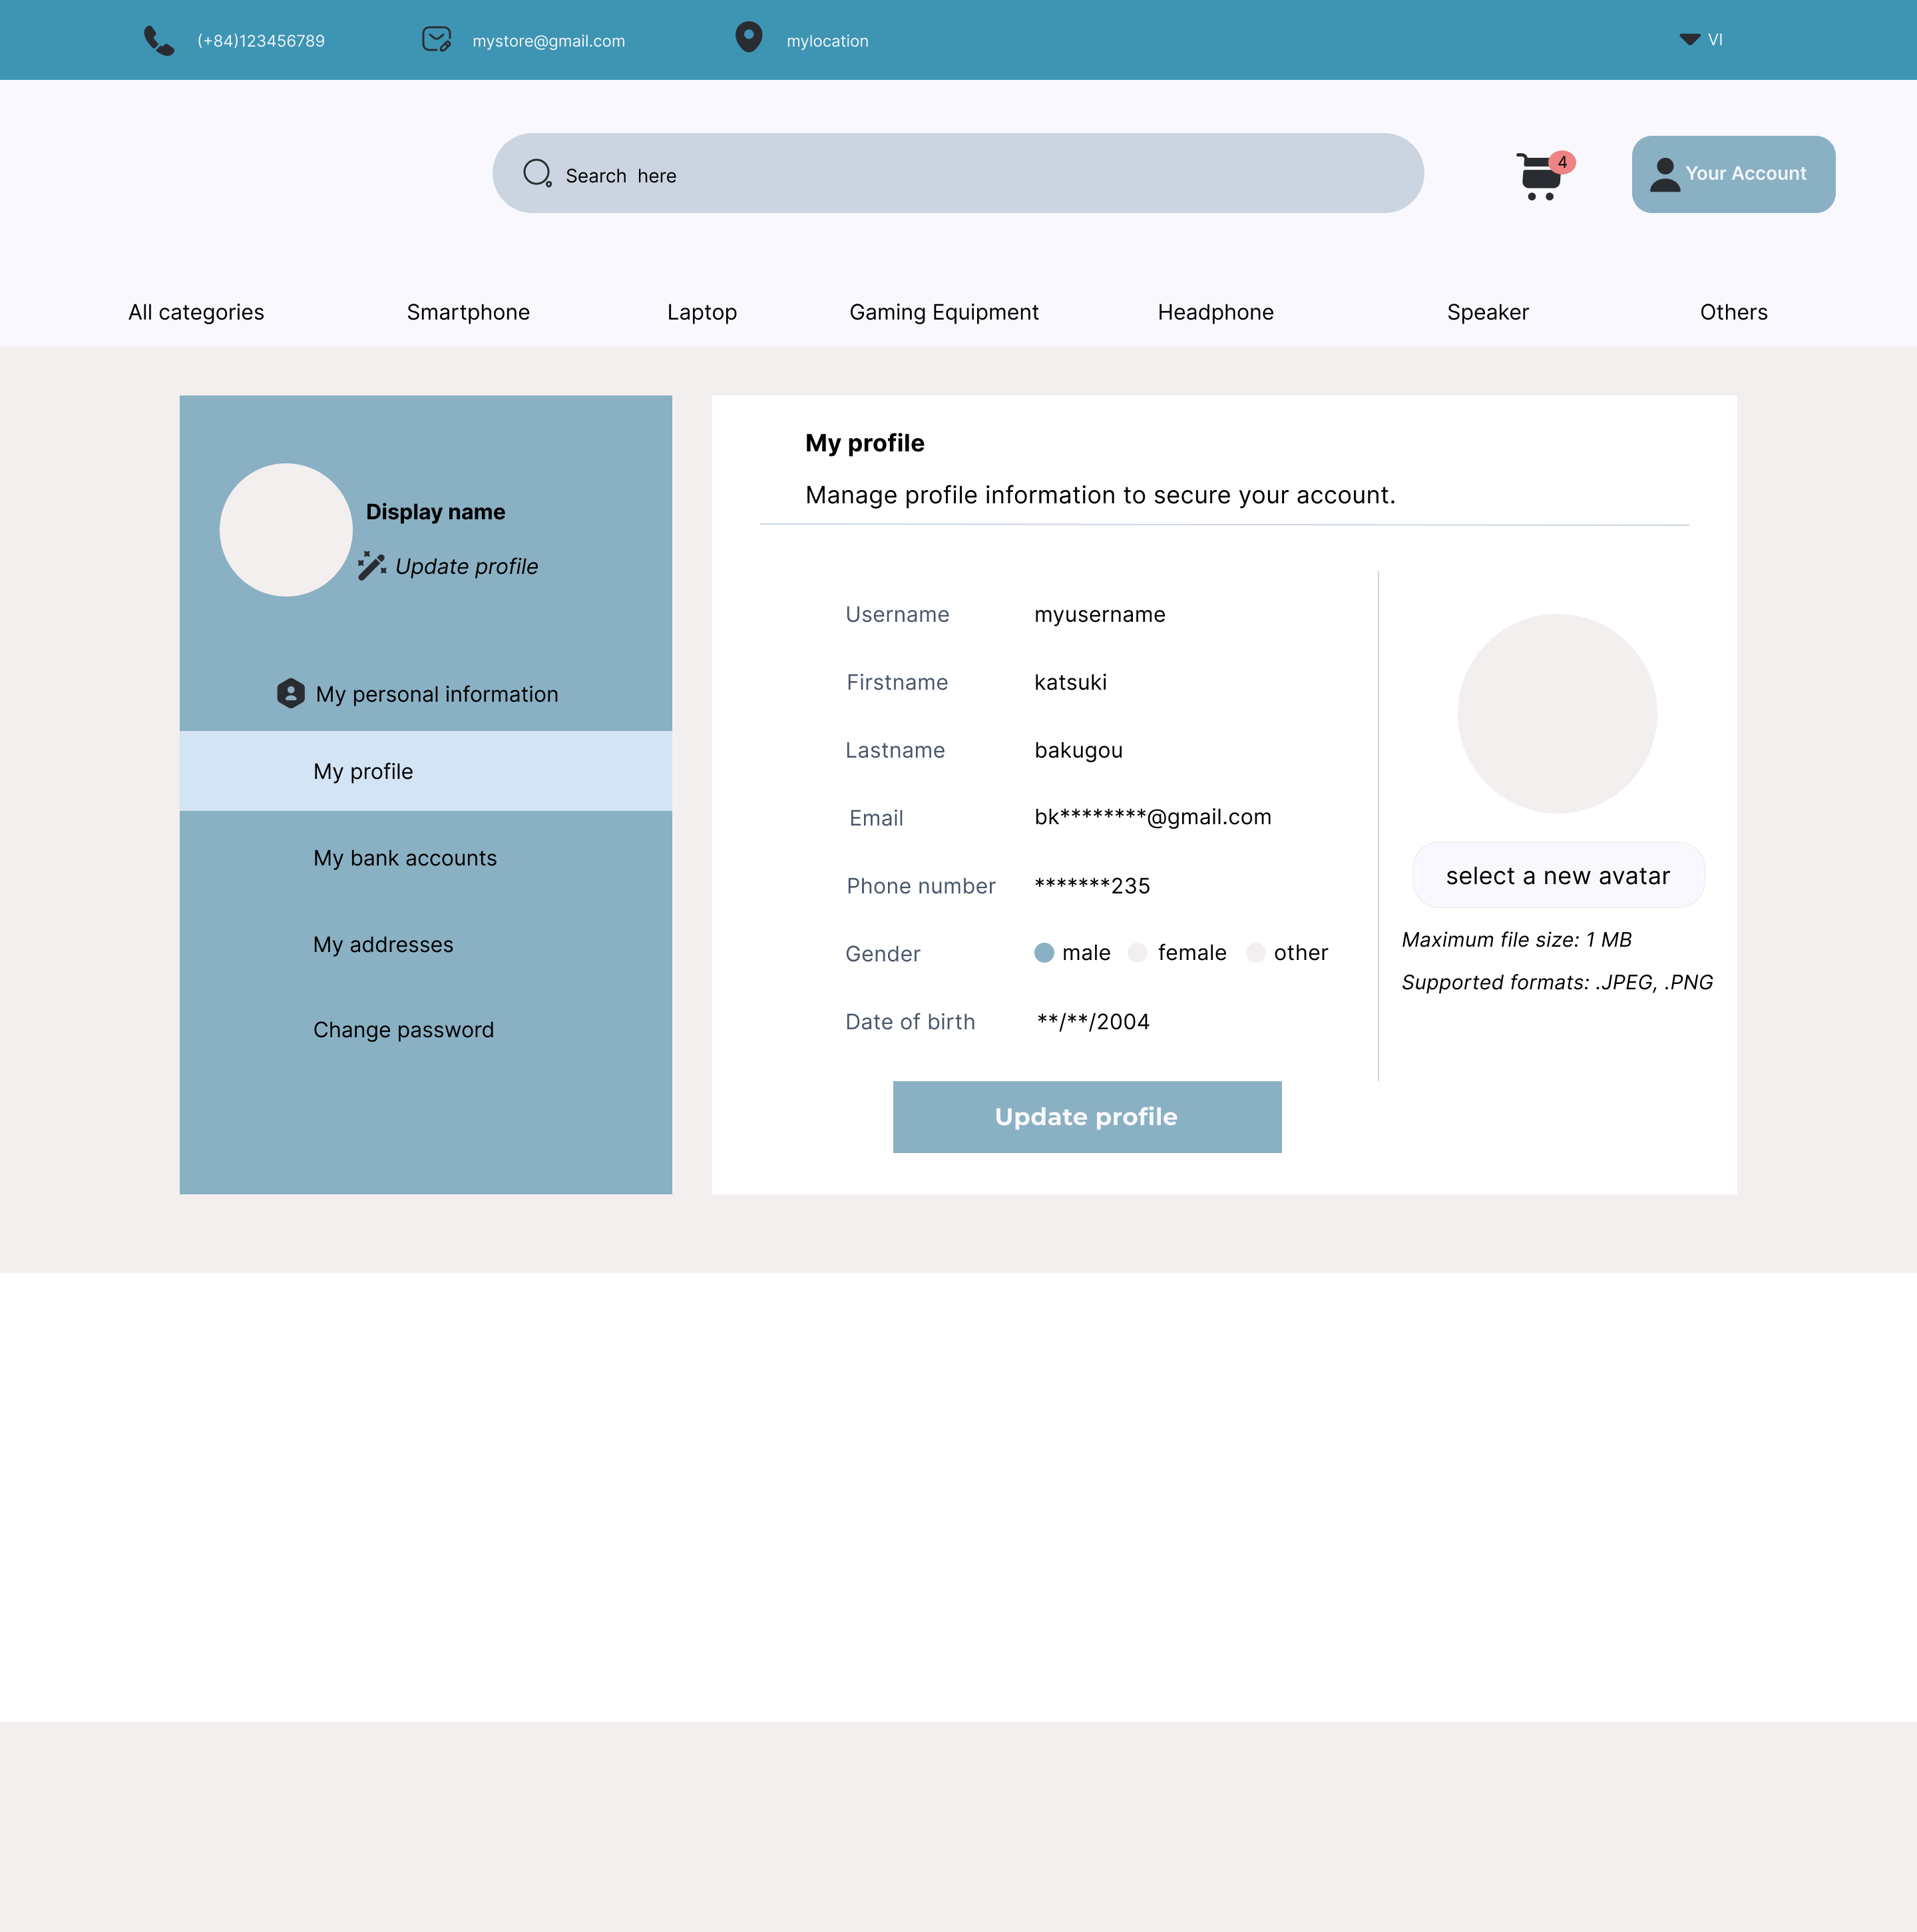
\includegraphics[width=0.8\linewidth]{images/chap6/ui/ui_view_profile_profile.png}
    \vspace{0.5cm}
    \caption{Giao diện Hồ sơ cá nhân}
    \label{fig:ui_profile_info}
\end{figure}
Giao diện hồ sơ cá nhân cho phép người dùng xem và cập nhật các thông tin cơ bản như họ tên, số điện thoại và email liên hệ. Đây là khu vực trung tâm để quản lý thông tin định danh và cá nhân hóa trải nghiệm sử dụng hệ thống.

% --- NHÓM 5: QUẢN LÝ ĐƠN HÀNG (USER) ---

\begin{figure}[H]
    \centering
    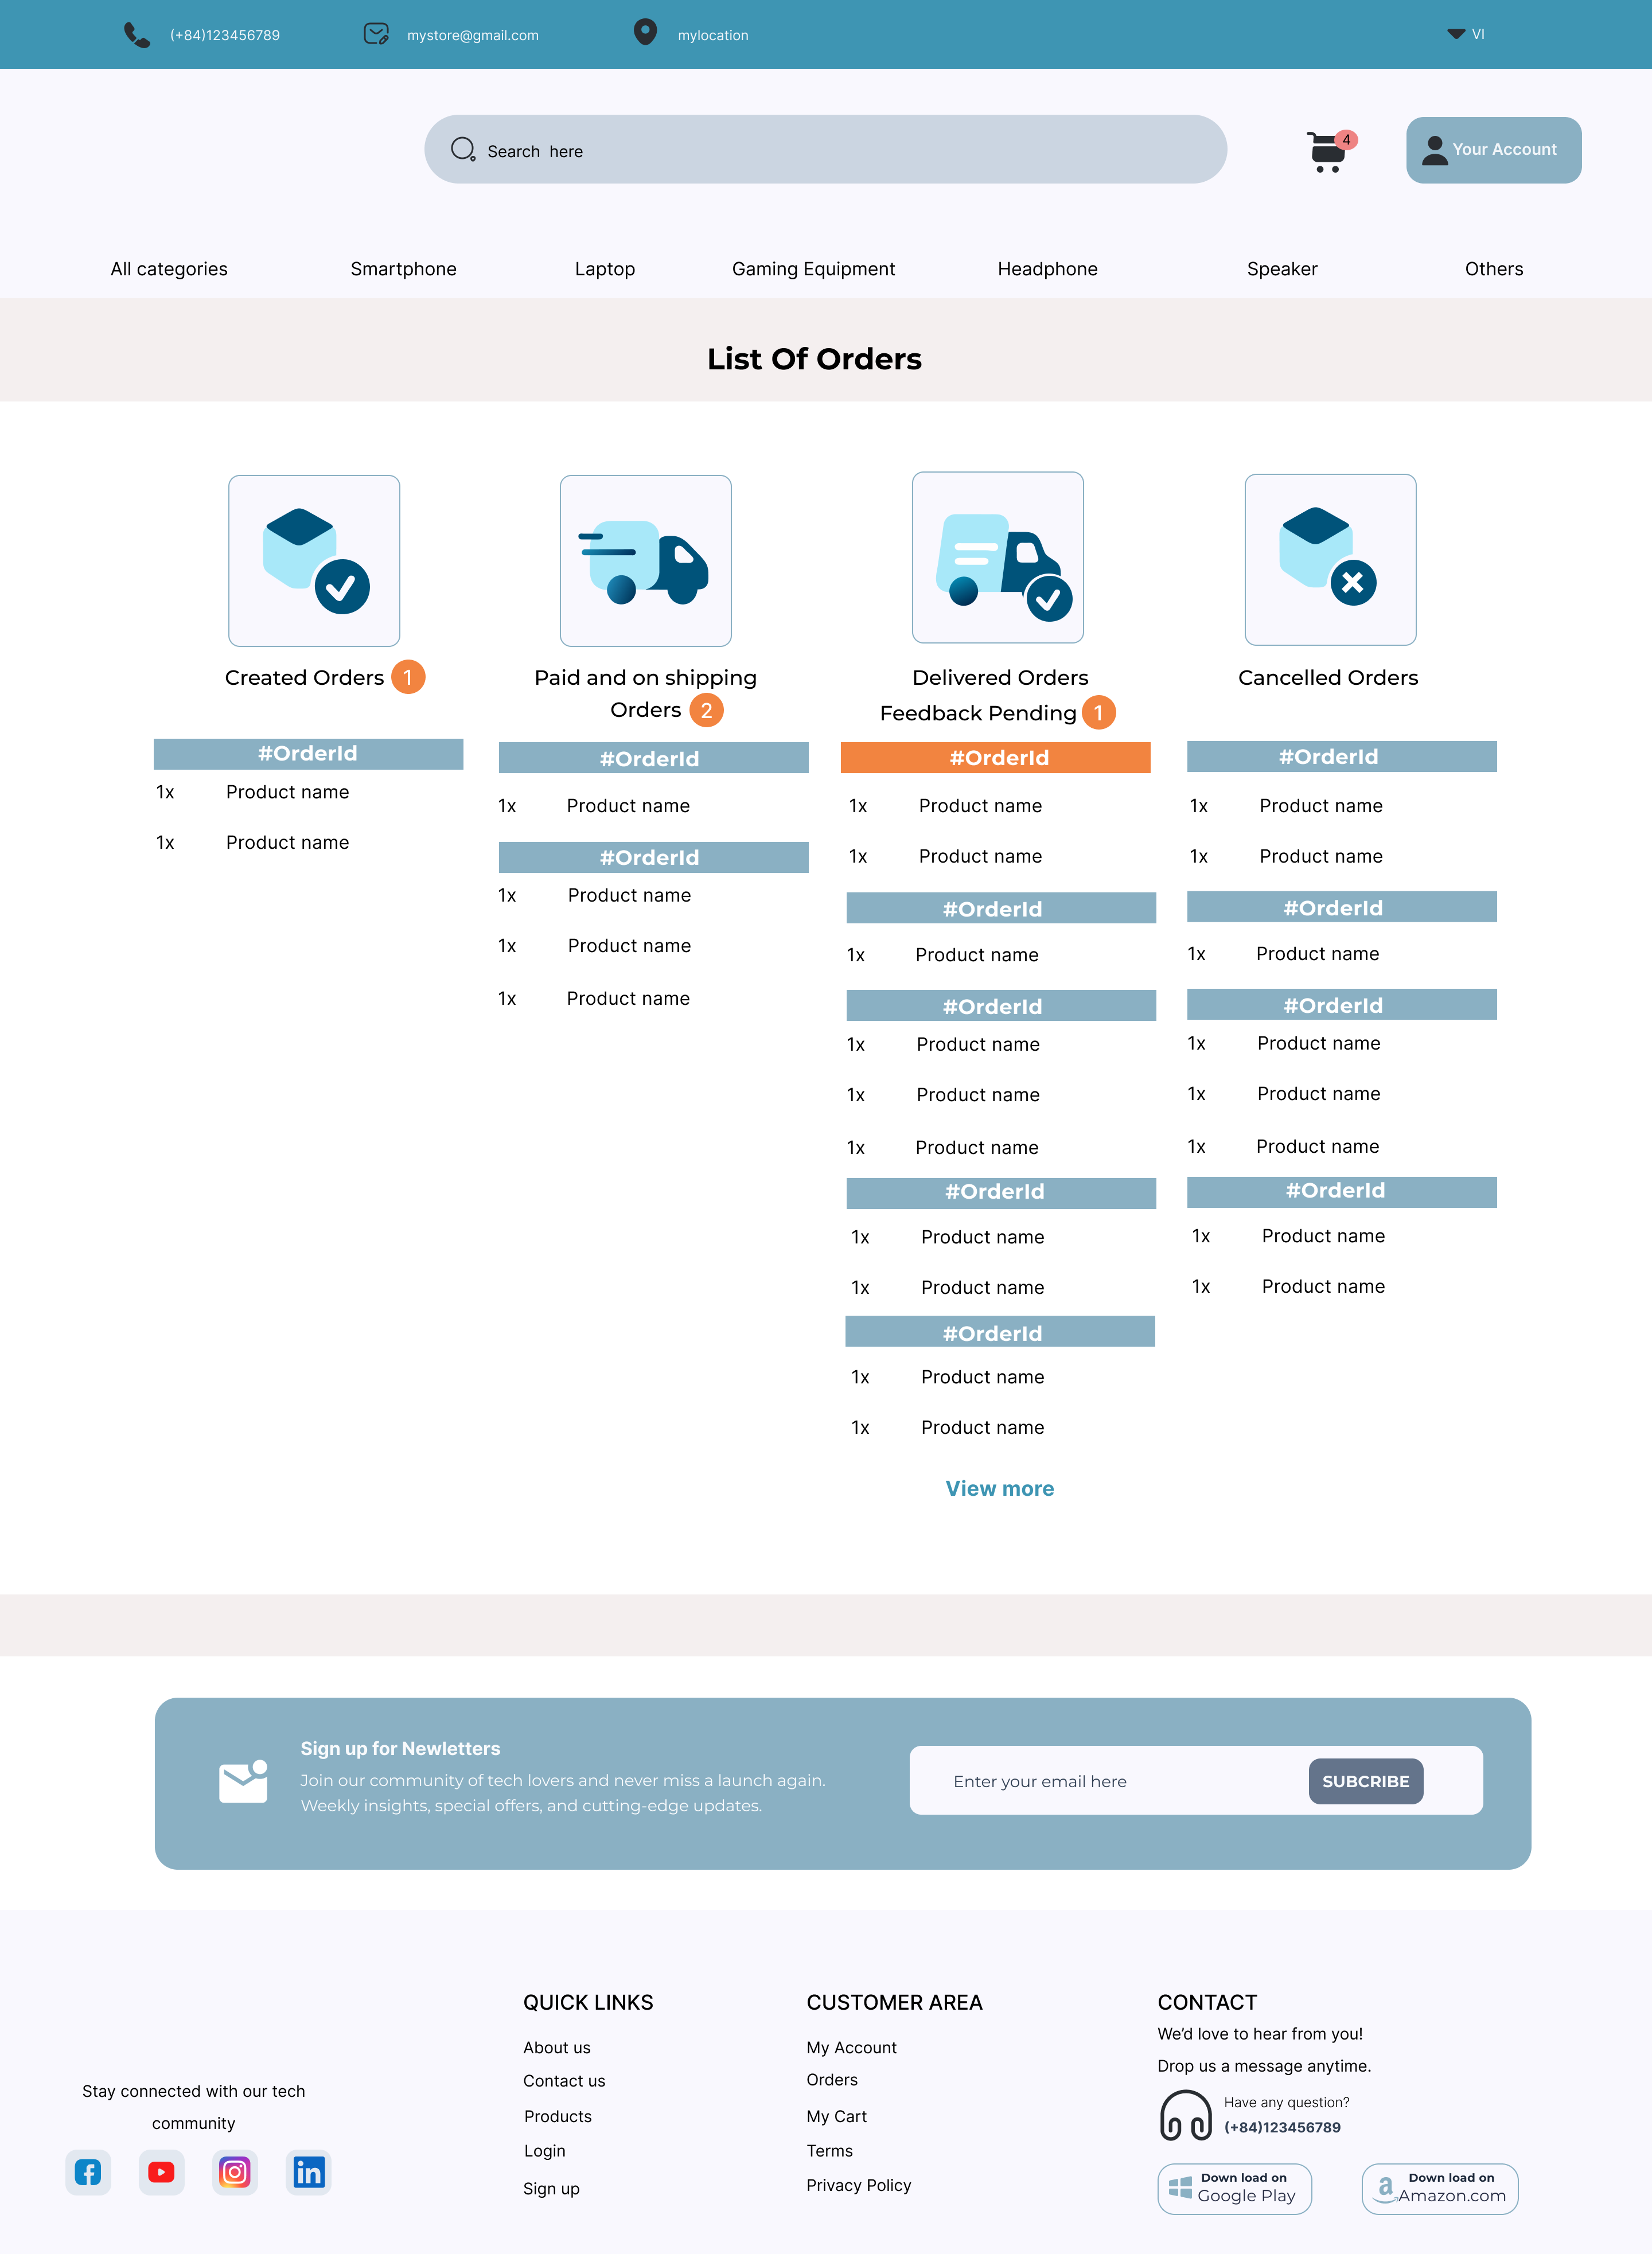
\includegraphics[width=0.9\linewidth]{images/chap6/ui/ui_list_of_order.png}
    \vspace{0.5cm}
    \caption{Giao diện Lịch sử đơn hàng}
    \label{fig:ui_order_list}
\end{figure}
Giao diện lịch sử đơn hàng liệt kê toàn bộ các đơn đã đặt, được phân loại theo trạng thái như chờ xác nhận, đang giao, đã giao hoặc đã hủy, giúp người dùng dễ dàng theo dõi tiến trình mua sắm.

\begin{figure}[H]
    \centering
    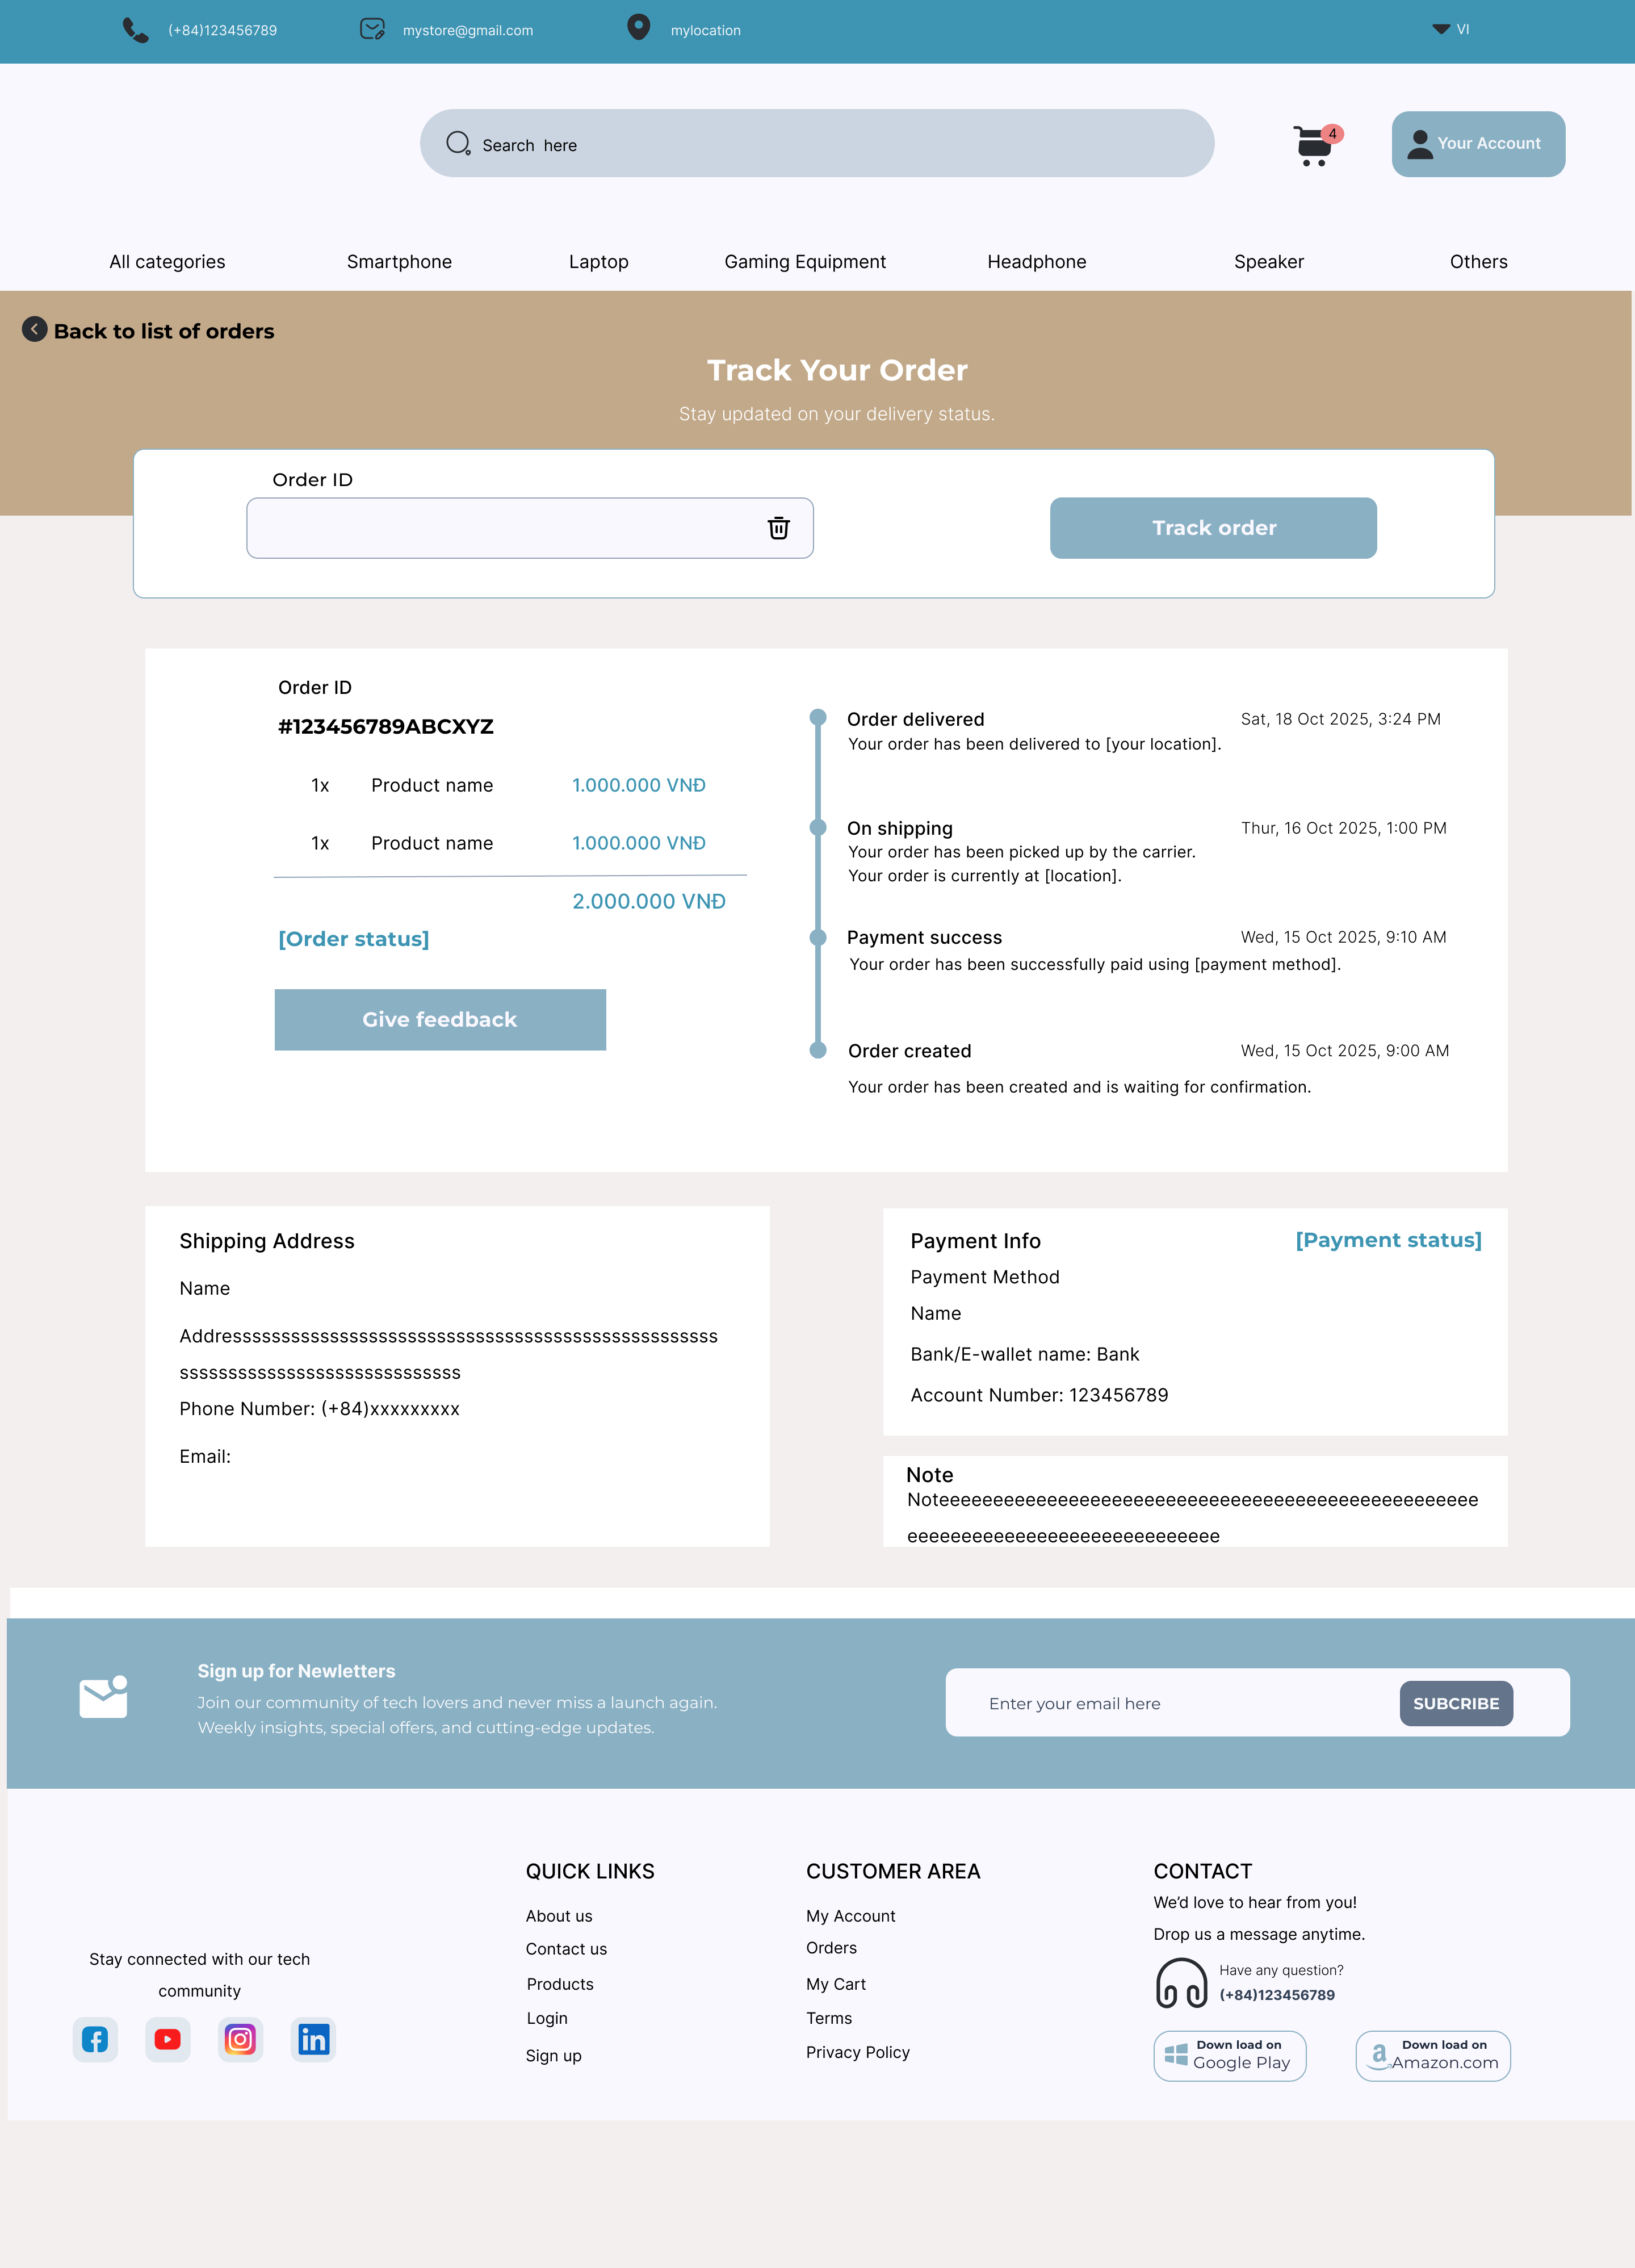
\includegraphics[width=0.9\linewidth]{images/chap6/ui/ui_tracking_order.png}
    \vspace{0.5cm}
    \caption{Giao diện Theo dõi đơn hàng}
    \label{fig:ui_tracking}
\end{figure}
Chức năng theo dõi đơn hàng sử dụng biểu đồ dòng thời gian để trực quan hóa các mốc xử lý quan trọng, từ lúc xác nhận đơn đến khi giao hàng thành công.

\subsubsection{Giao diện quản trị}

\begin{figure}[H]
    \centering
    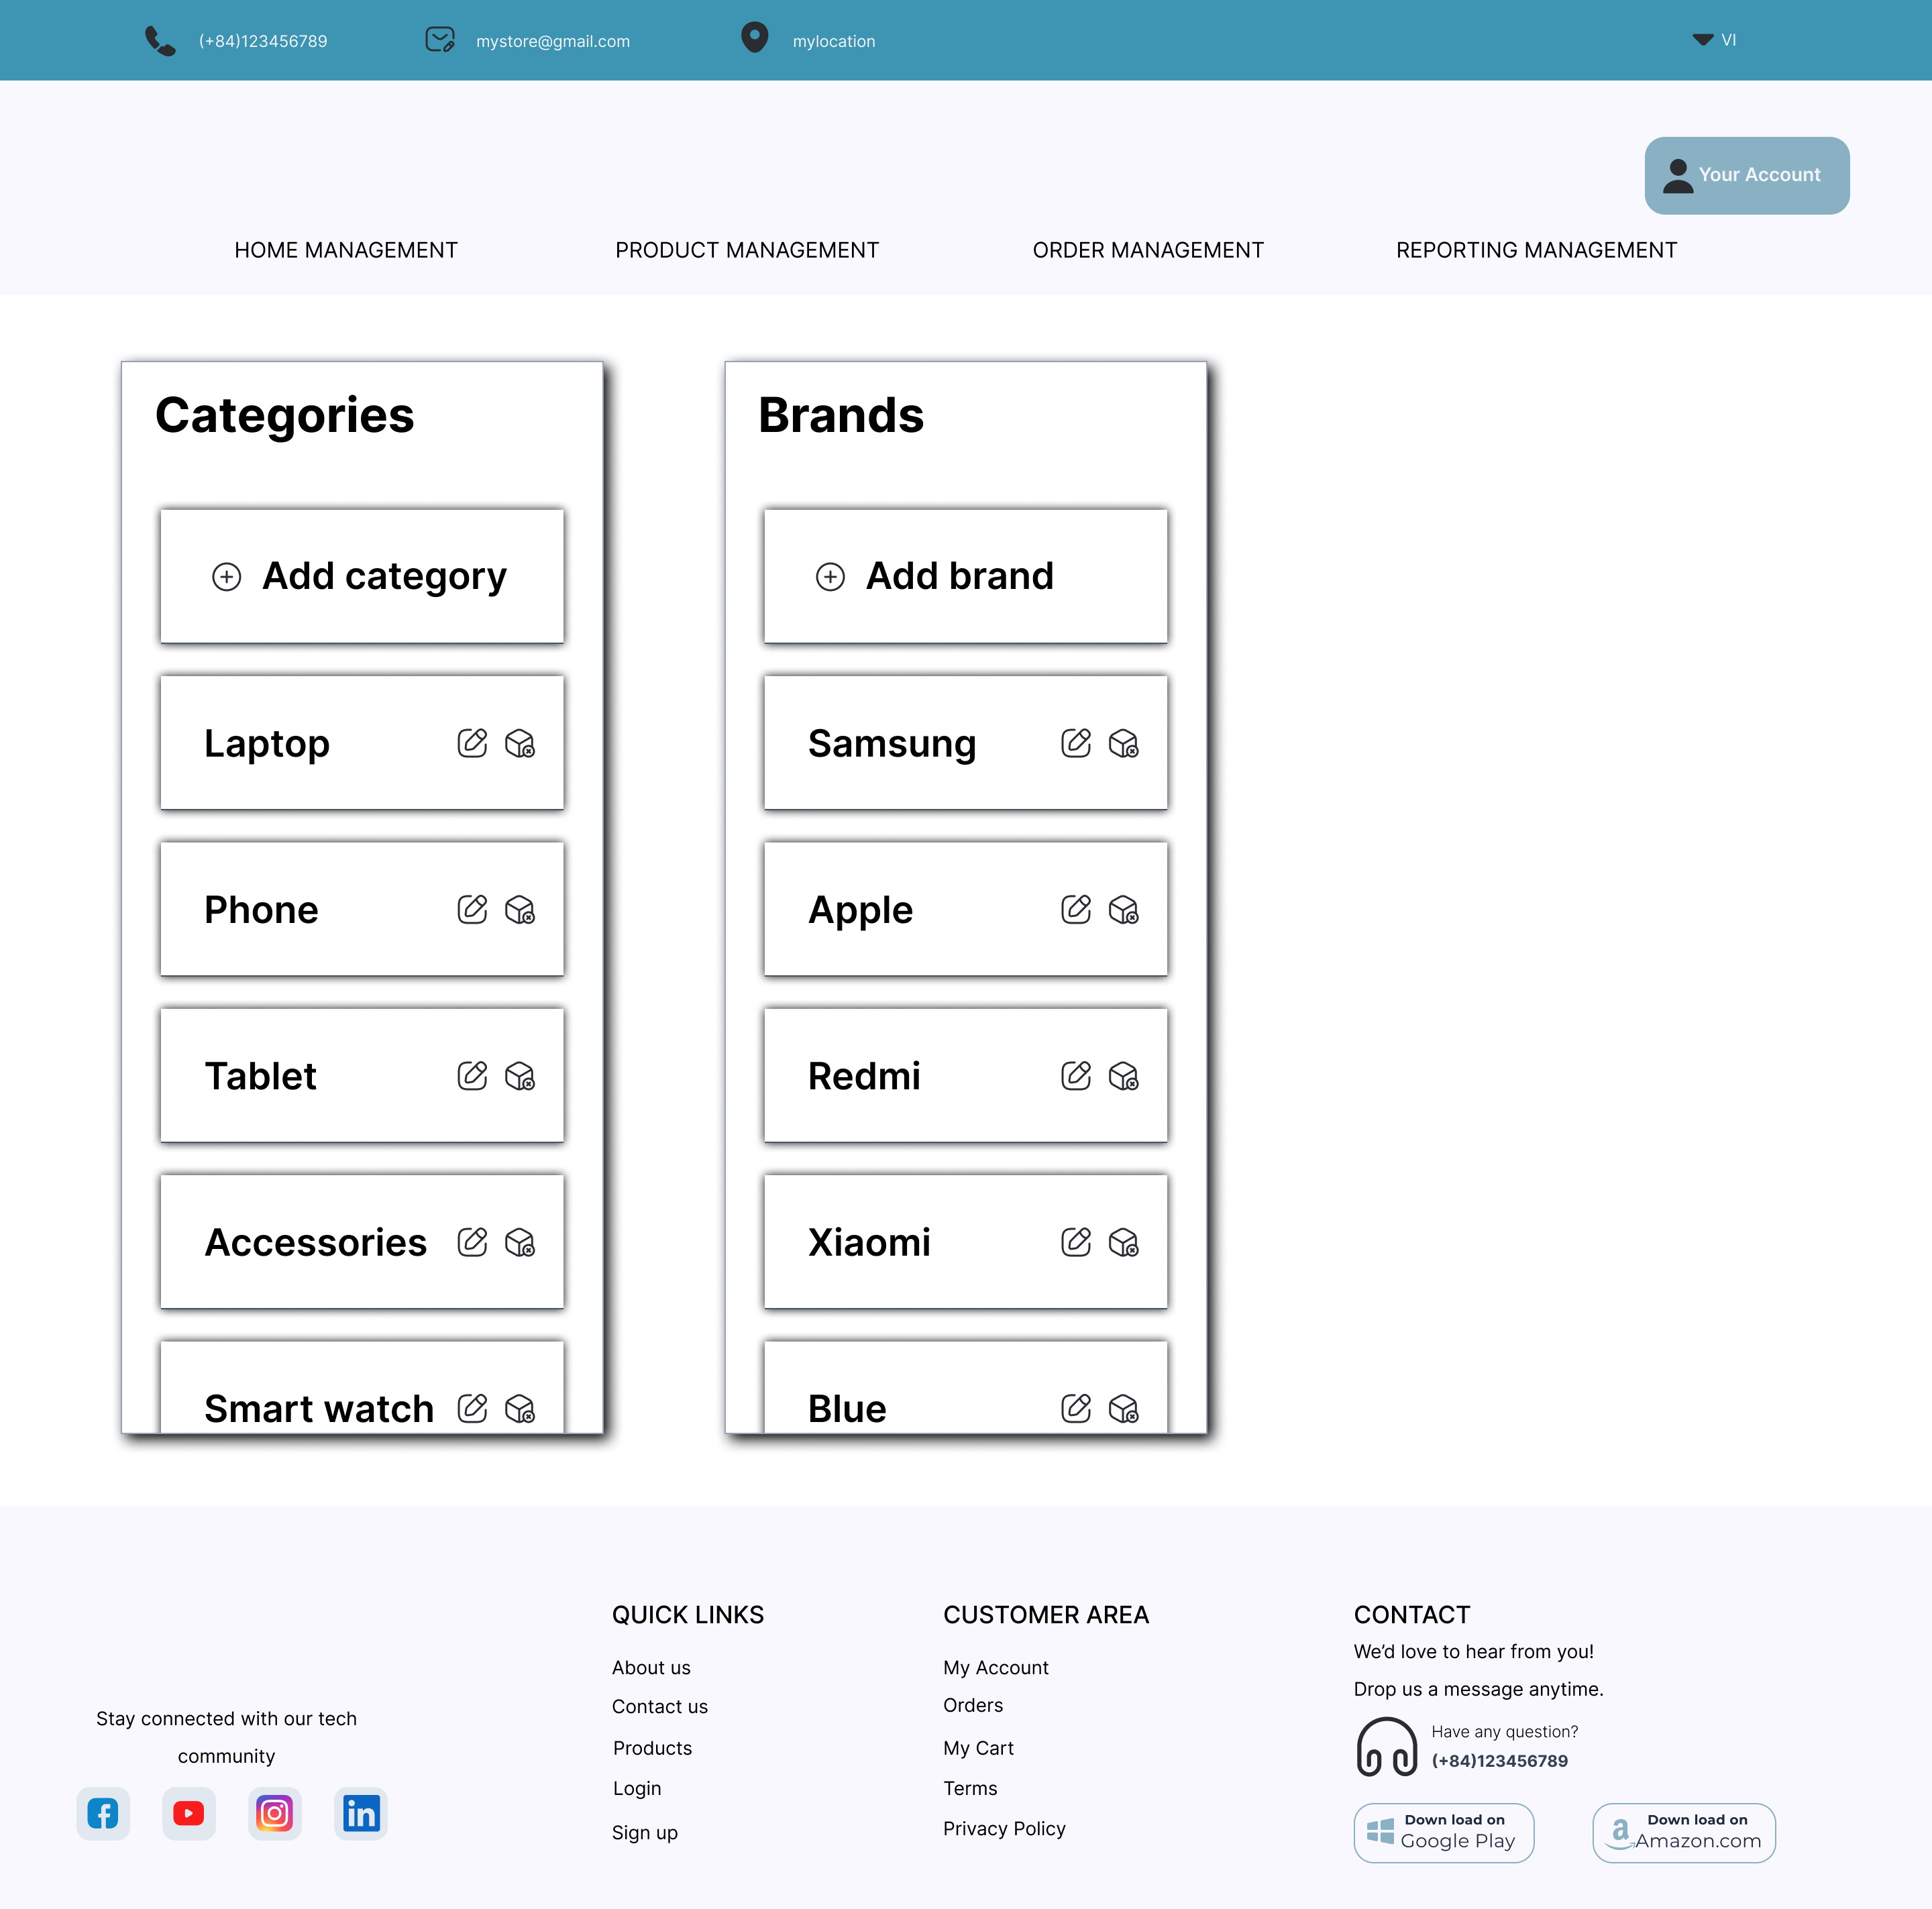
\includegraphics[width=1.0\linewidth]{images/chap6/ui/ui_admin_home.png}
    \vspace{0.5cm}
    \caption{Giao diện Dashboard quản trị}
    \label{fig:ui_admin_home}
\end{figure}
Dashboard quản trị cung cấp cái nhìn tổng quan về tình hình hoạt động của hệ thống thông qua các chỉ số kinh doanh quan trọng như doanh thu, số lượng đơn hàng và số người dùng mới.

\begin{figure}[H]
    \centering
    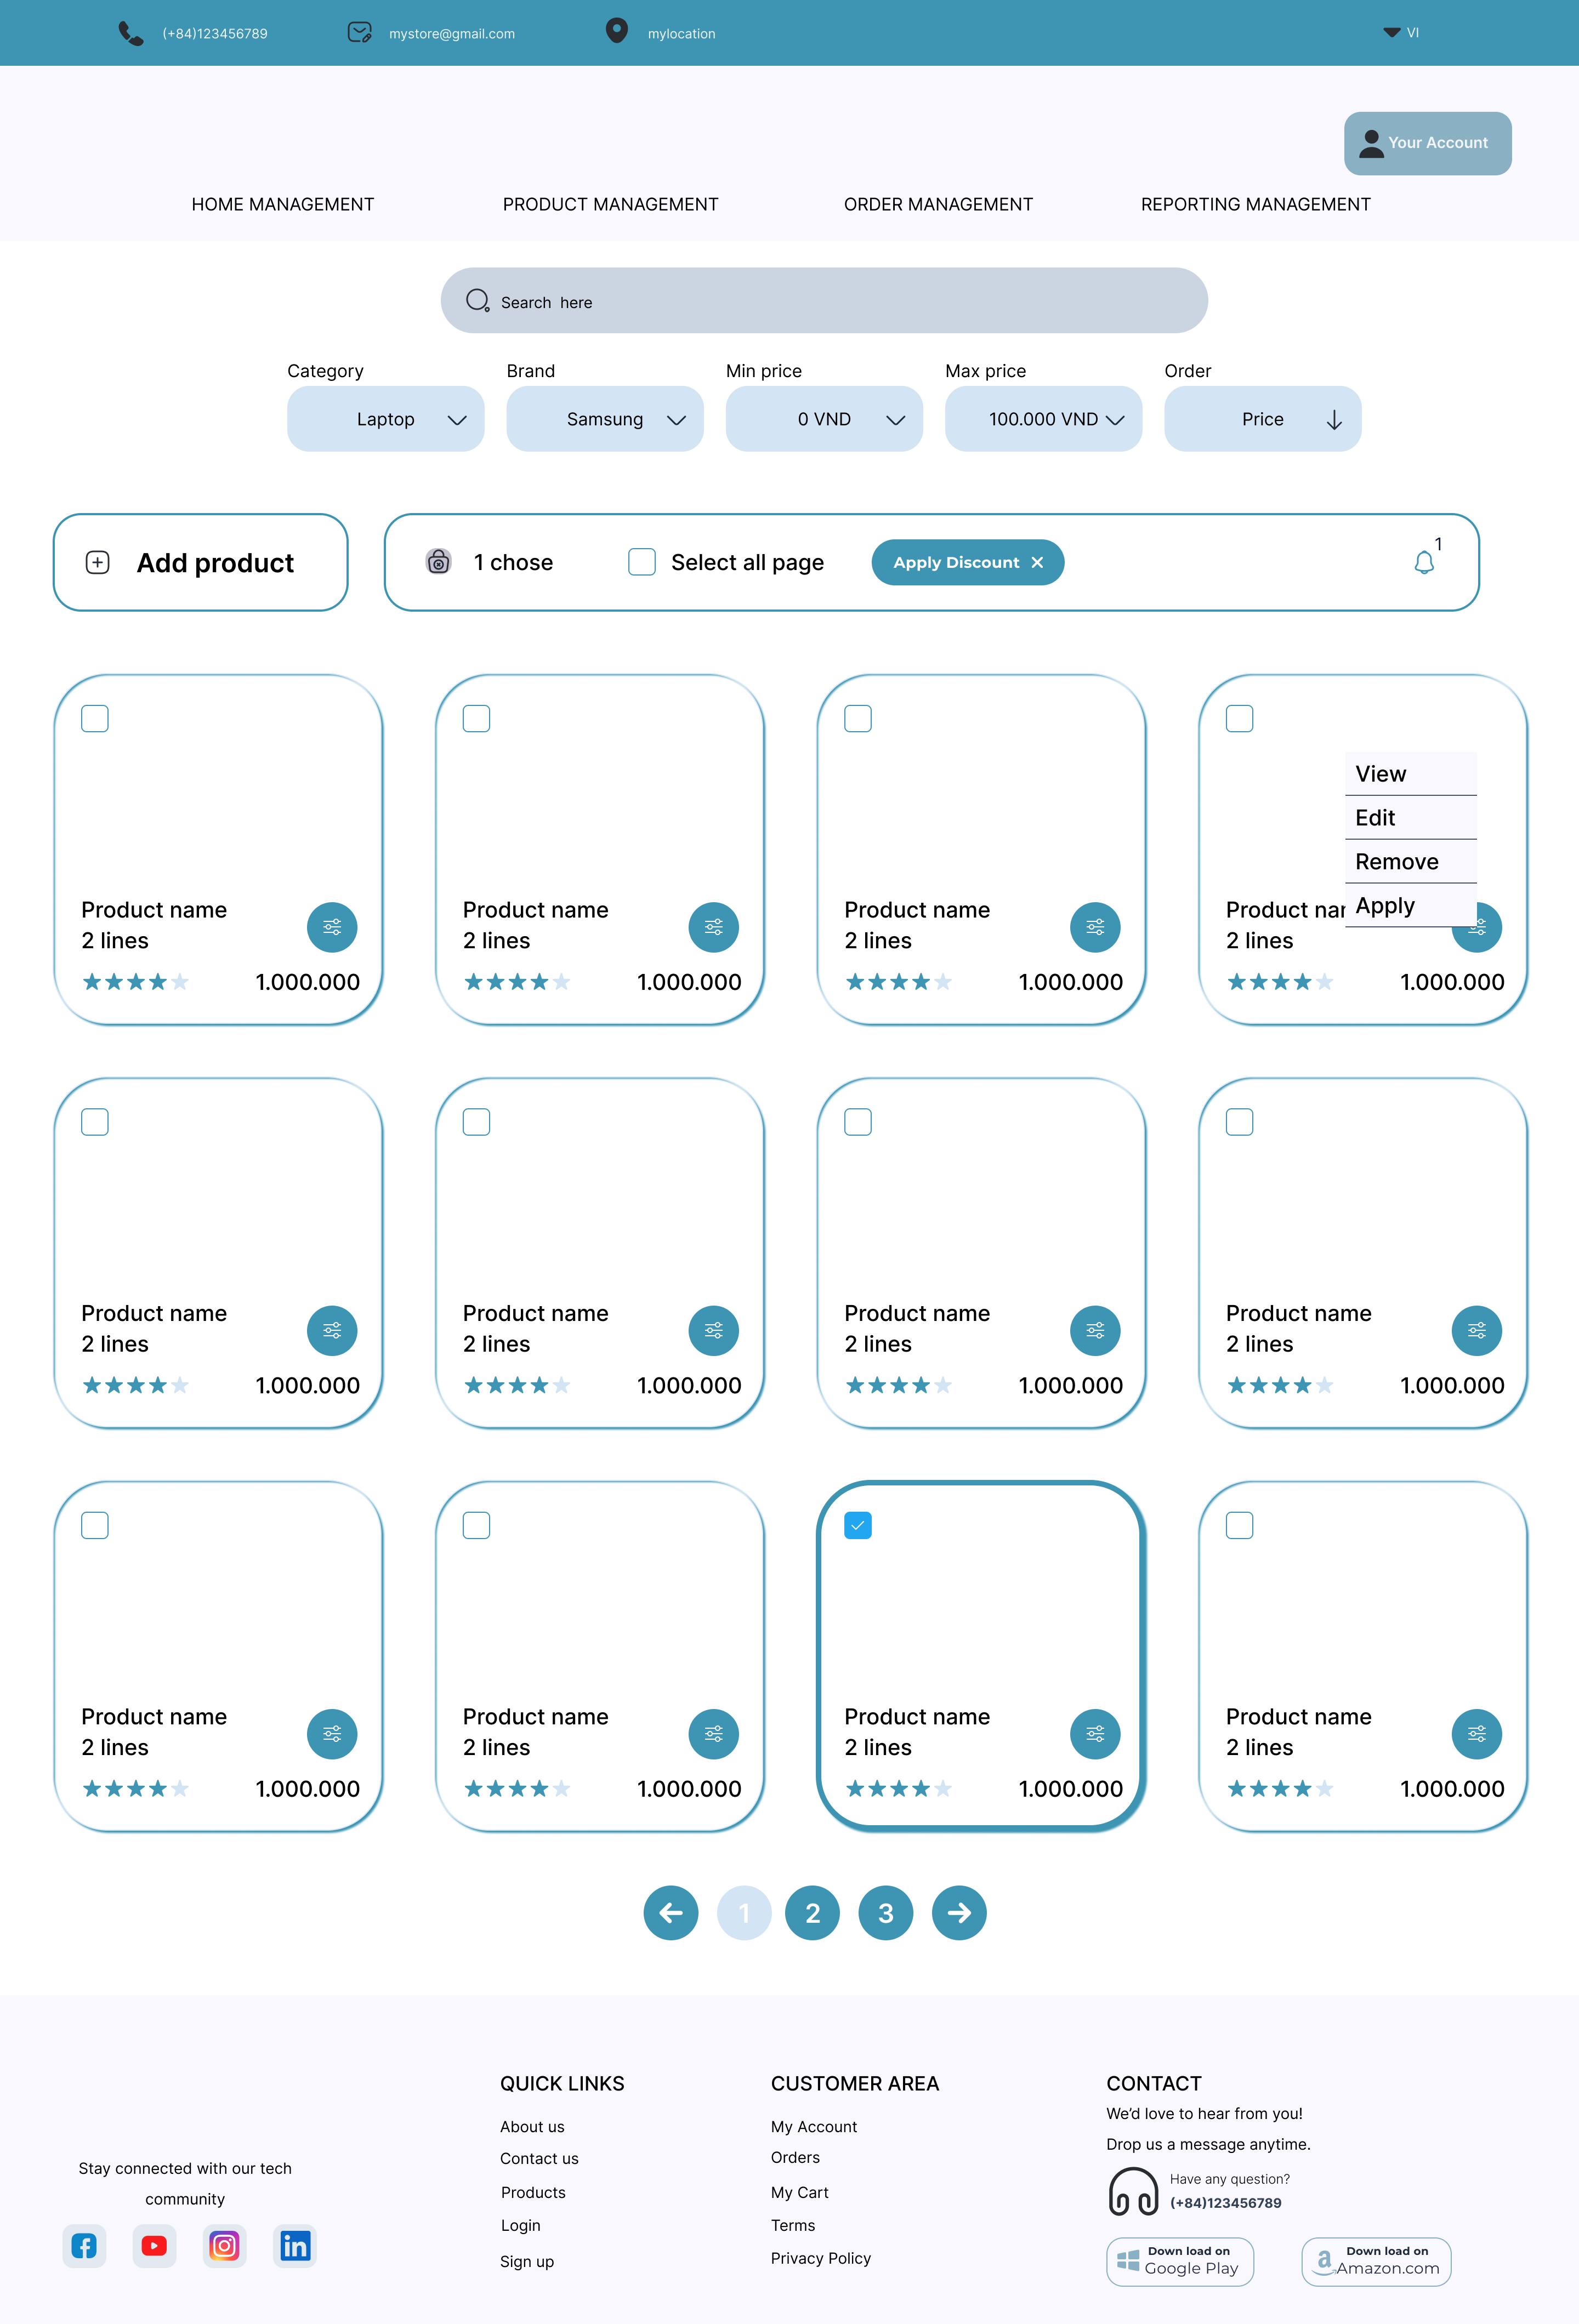
\includegraphics[width=1.0\linewidth]{images/chap6/ui/ui_admin_product.png}
    \vspace{0.5cm}
    \caption{Giao diện Quản lý sản phẩm}
    \label{fig:ui_admin_product}
\end{figure}
Giao diện quản lý sản phẩm cho phép quản trị viên thực hiện các thao tác thêm, sửa, xóa sản phẩm, cập nhật giá bán và quản lý tồn kho nhằm đảm bảo dữ liệu sản phẩm luôn chính xác.

\begin{figure}[H]
    \centering
    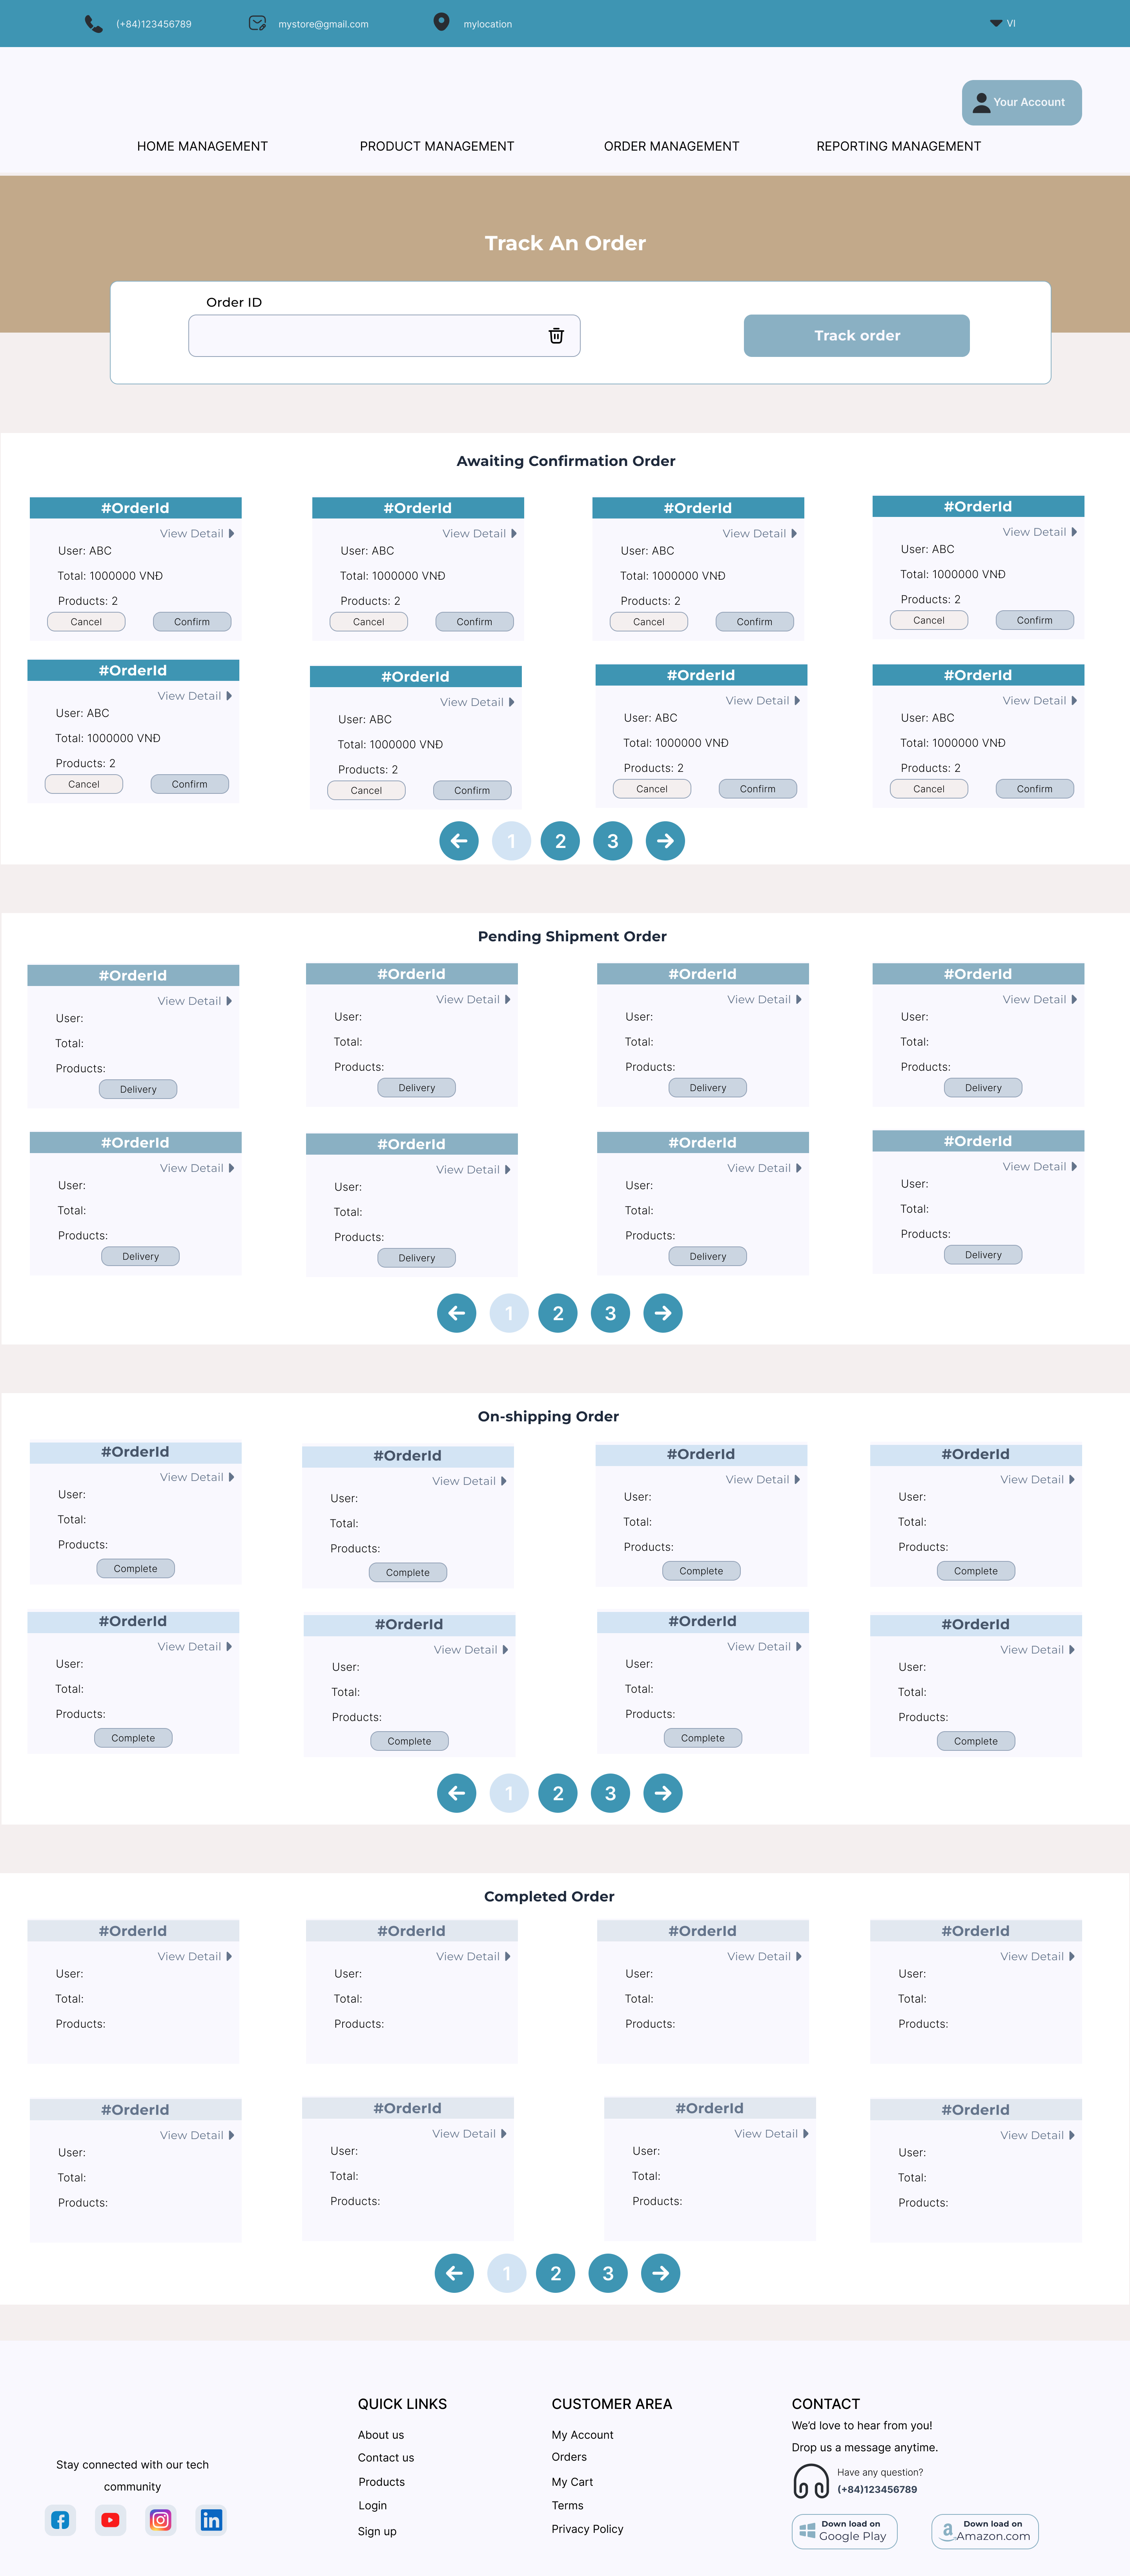
\includegraphics[width=0.6\linewidth]{images/chap6/ui/ui_order_management.png}
    \vspace{0.5cm}
    \caption{Giao diện Quản lý đơn hàng}
    \label{fig:ui_admin_orders}
\end{figure}
Trang quản lý đơn hàng hỗ trợ quản trị viên theo dõi và xử lý toàn bộ đơn hàng trên hệ thống, cho phép lọc theo trạng thái để phục vụ các nghiệp vụ vận hành như duyệt đơn, đóng gói và giao hàng.
